\documentclass[12pt]{article}
\usepackage{indentfirst}
\usepackage[utf8x]{inputenc}
\usepackage[T1]{fontenc}
\usepackage[english,lithuanian]{babel}
\usepackage{array}
\usepackage{caption}
\usepackage{subcaption}
\usepackage{makecell}
\usepackage[euler]{textgreek}
\usepackage{multirow}
\usepackage{boldline}
\usepackage{floatrow}
\floatsetup[table]{capposition=top}
\usepackage{amsmath, amsthm, amssymb}
\usepackage{graphicx}
\usepackage{setspace}
\usepackage{verbatim}
\usepackage[left=3cm,top=2cm,right=1.5cm,bottom=2cm]{geometry}
\usepackage{floatrow}
\newfloatcommand{capbtabbox}{table}[][\FBwidth]
\usepackage{blindtext}
\onehalfspacing
\usepackage[hidelinks, unicode]{hyperref}
\usepackage{textcomp}
\usepackage{amsmath}
\usepackage{cleveref}
\usepackage[labelfont=bf]{caption}
\usepackage{microtype}
\usepackage{tabularx}
\captionsetup[table]{font={normalfont},format=plain,labelsep=period}
\graphicspath{{../assets/images/}}
\usepackage[table]{xcolor}
\definecolor{newGray}{rgb}{0.878, 0.878, 0.878}
\usepackage{longtable}
\usepackage{enumitem}
\definecolor{deepchampagne}{rgb}{0.98, 0.84, 0.65}
\definecolor{dartmouthgreen}{rgb}{0.09, 0.45, 0.27}
\definecolor{deepcarmine}{rgb}{0.66, 0.13, 0.24}
\usepackage{makecell}

\newcommand{\EE}{\mathbb{E}\,}
\newcommand{\ee}{{\mathrm e}}
\newcommand{\dd}{{\mathrm d}}
\newcommand{\RR}{\mathbb{R}}

\begin{document}
\selectlanguage{lithuanian}

\begin{titlepage}
\vskip 20pt
\begin{center}
\includegraphics[scale=1.4]{KTU.png}
\end{center}

%%%%%%%%%%%%%%%%%%%%%%%
% TITULINIS PUSLAPIS
%%%%%%%%%%%%%%%%%%%%%%%

\vskip 20pt
\centerline{\bf \large \textbf{Kauno technologijos universitetas}}
\bigskip
\centerline{\large {Informatikos fakultetas}}
\bigskip

\vskip 90pt
\begin{center}
    {\bf \LARGE Modulis „Tiriamasis projektas 2“}
    \vskip 10pt
    {\bf \Large Projektas: „Savarankiškos suverenios pseudonimizuotos tapatybės 
    valdymo sistema“}
    \vskip 15pt
    {\large Reikalavimų specifikavimas}
\end{center}

\vskip 40pt

\hskip 200pt {\bf \large IFM 4/2 gr. Danielė Stasiūnaitė}
\vskip 1pt
\hskip 200pt {\large Studentė}
\vskip 7pt
\hskip 200pt {\bf \large Doc. Mindaugas Vasiljevas}
\vskip 1pt
\hskip 200pt {\large Projekto vadovas}
\vskip 7pt
\hskip 200pt {\bf \large Doc. dr. Eglė Butkevičiūtė}
\vskip 1pt
\hskip 200pt {\large Dėstytoja}

\bigskip

\vskip 100pt
\centerline{\large \textbf{Kaunas, 2025}}
\newpage
\end{titlepage}

\selectlanguage{lithuanian}

%%%%%%%%%%%%%%%%%%%%%
% TURINIO PUSLAPIS
%%%%%%%%%%%%%%%%%%%%%

\tableofcontents
\newpage

\section{Sistemos paskirtis}
\subsection{Projekto kūrimo pagrindas (pagrindimas)}
Skaitmeniniame amžiuje, kai asmens duomenys tampa viena svarbiausių vertybių,
privatumo užtikrinimas ir efektyvus tapatybės valdymas yra pagrindiniai
iššūkiai, su kuriais turi susidurti ne tik privatūs asmenys, bet ir įvairios
organizacijos. Sparčiai augantys informacijos srautai, elektroninių paslaugų
plėtra bei kitų paslaugų, reikalaujančių naudotojų autentifikacijos, vystymas
lėmė inovatyvių technologinių sprendimų - blokų grandinės pritaikymo, 
realizuojant decentralizuotos asmens tapatybės valdymo modelį - kūrimą.
Pastaruoju sprendimu siekiama užtikrinti asmens duomenų saugumą bei visapusišką
duomenų kontrolę, kuri atliekama paties naudotojo.

Šiuo metu egzistuojančios asmens tapatybės valdymo sistemos, pavyzdžiui,
centralizuotos ar federacinės, dažnai susiduria su privatumo, duomenų apsaugos
ir patogumo iššūkiais. Centralizuotos sistemos yra itin jautrios saugumo
pažeidimams, o federacinės sistemos dažnai riboja naudotojo autonomiją. Šie
trūkumai skatina naujų sprendimų kūrimo poreikį, orientuotą į naudotojo teisių
ir privatumo stiprinimą.

Šis projektas skirtas sukurti savarankiškos suverenios pseudonimizuotos
tapatybės valdymo sistemą, kuri leistų naudotojams
ne tik valdyti asmeninę informaciją ir dalinimąsi ja, bet ir užtikrintų, kad
asmeniniai duomenys negalėtų būti lengvai susieti su naudotoju, kurį šie
duomenys apibūdina. Šie tikslai bus pasiekti, pritaikius decentralizuotos
tapatybės valdymo modelį, kuris grindžiamas blokų grandinės technologija,
duomenų šifravimo bei pseudonimizavimo metodikomis.

\subsection{Sistemos tikslai (paskirtis)}
Sistemos kūrimo projektu siekiama įgyvendinti šiuos tikslus:
\begin{itemize}
    \item 1
    \item 2
    \item 3
    \item 4
    \item 5
\end{itemize}

\section{Užsakovai, pirkėjai ir kiti sistema suinteresuoti asmenys}
\subsection{Užsakovas}
Sistemos kūrimo projektą užsako darbo vadovas Mindaugas Vasiljevas. Užsakovo
rolės projekte apima sistemos finansavimo, reikalavimų sistemai rinkimo ir
teikimo bei konsultacijų, susijusių su dalykine sritimi, teikimą.
Darbo vadovo kontaktiniai duomenys:

\begin{table}[htb!]
    \captionsetup{justification=centering}
    \caption{\small\textbf{Panaudojimo atvejo specifikacija Nr.2.}}
    \begin{tabular}{|m{6cm}|m{11cm}|}
        \hline
        \raggedleft \textbf{\cellcolor{deepchampagne}Mobilusis telefonas:} &
        +37066428763. \\
        \hline
        \raggedleft \textbf{\cellcolor{deepchampagne}El. pašto adresas} &
        mindaugas.vasiljevas@ktu.lt. \\
        \hline
        \raggedleft \textbf{\cellcolor{deepchampagne}Adresas} & 
        XI rūmai 3C2b korpusas. \\
        \hline
        \raggedleft \textbf{\cellcolor{deepchampagne}Informacijos galima teirautis}
        & I - V; 10:00 - 17:00. \\
        \hline
    \end{tabular}
    \label{table:kontaktiniai_duomenys}
\end{table}

\subsection{Pirkėjas}
Sistemos pirkėjas sutampa su sistemos užsakovu.

\subsection{Naudotojai}
Žemiau yra pateikiami potencialių sistemos naudotojų - pacientų, gydytojų ir
tyrėjų - aprašymai kartu su šių naudotojų charakteristikomis.

\subsubsection*{Pacientai}
\label{sec:N1}
\begin{table}[htb!]
    \captionsetup{justification=centering}
    \vskip -10pt
    \begin{tabular}{|m{4cm}|m{12cm}|}
        \hline
        \raggedleft \textbf{\cellcolor{deepchampagne}Funkcijos} &
        Valdyti savo asmeninių genetinių duomenų prieinamumą kitoms naudotojų
        grupėms; esant poreikiui, įkelti genetinius duomenis; peržiūrėti
        analizių, atliktų su genetiniais duomenimis, rezultatus. \\
        \hline
        \raggedleft \textbf{\cellcolor{deepchampagne}Patirtis dalykinėje
        srityje} & Žema. \\
        \hline
        \raggedleft \textbf{\cellcolor{deepchampagne}Patirtis IT srityje} &
        Žema. \\
        \hline
        \raggedleft \textbf{\cellcolor{deepchampagne}Papildomos
        charakteristikos} &
        Sistema besinaudojančius
        pacientus sieja kalba (lietuvių kalba) ir interesai (valdyti savo
        asmeninius genetinius duomenis, kurie gali būti panaudoti, net tik
        atliekant asmens genetinius tyrimus, bet ir moksliniais tikslais). \\
        \hline
        \raggedleft \textbf{\cellcolor{deepchampagne}Prioritetas} & Aukštas. \\
        \hline
    \end{tabular}
\end{table}

\newpage

\subsubsection*{Gydytojai - genetikai}
\label{sec:N2}
\begin{table}[htb!]
    \captionsetup{justification=centering}
    \vskip -10pt
    \begin{tabular}{|m{4cm}|m{12cm}|}
        \hline
        \raggedleft \textbf{\cellcolor{deepchampagne}Funkcijos} &
        Įkelti pacientų genetinius duomenis; atlikti genetinių duomenų analizes
        ir jų rezultatus pateikti pacientams; gavus leidimą iš paciento perduoti
        genetinius duomenis tyrėjams. \\
        \hline
        \raggedleft \textbf{\cellcolor{deepchampagne}Patirtis dalykinėje
        srityje} & Aukšta. \\
        \hline
        \raggedleft \textbf{\cellcolor{deepchampagne}Patirtis IT srityje} &
        Vidutinė. \\
        \hline
        \raggedleft \textbf{\cellcolor{deepchampagne}Papildomos
        charakteristikos} &
        Gydytojus - genetikus sieja išsilavinimas (aukštasis - universitetinis),
        darbo pobūdis (pacientų genetinių duomenų apdorojimas) ir dalykinė
        sritis (sveikatos priežiūra). \\
        \hline
        \raggedleft \textbf{\cellcolor{deepchampagne}Prioritetas} & Aukštas. \\
        \hline
    \end{tabular}
\end{table}

\subsubsection*{Tyrėjai}
\label{sec:N3}
\begin{table}[htb!]
    \captionsetup{justification=centering}
    \vskip -10pt
    \begin{tabular}{|m{4cm}|m{12cm}|}
        \hline
        \raggedleft \textbf{\cellcolor{deepchampagne}Funkcijos} &
        Atlikti išsamesnes genetinių duomenų analizes (genetinius duomenis
        apdorojant su specializuotais įrankiais) ir jų rezultatus pateikti
        gydytojams - genetikams. \\
        \hline
        \raggedleft \textbf{\cellcolor{deepchampagne}Patirtis dalykinėje
        srityje} & Aukšta. \\
        \hline
        \raggedleft \textbf{\cellcolor{deepchampagne}Patirtis IT srityje} &
        Aukšta. \\
        \hline
        \raggedleft \textbf{\cellcolor{deepchampagne}Papildomos
        charakteristikos} &
        Tyrėjus sieja išsilavinimas (aukštasis - universitetinis), darbo pobūdis
        (pacientų genetinių duomenų apdorojimas) ir dalykinė sritis (moksliniai
        tyrimai). \\
        \hline
        \raggedleft \textbf{\cellcolor{deepchampagne}Prioritetas} & Aukštas. \\
        \hline
    \end{tabular}
\end{table}

\newpage

\section{Apribojimai}
\subsection{Apribojimai sprendimui}
Kuriama sistema turi būti kuriama Windows 10 ar vėlesnių operacinės sistemos
versijų pagrindu.

\subsection{Diegimo aplinka}

\subsection{Komunikuojančios sistemos}
Sistemos komunikacija su gretimomis sistemomis nėra numatyta.

\subsection{Komerciniai specializuoti programų paketai}
Užsakovo nurodymu kuriama sistema turi veikti reliacinės duomenų bazės valdymo
sistemos Microsoft Server pagrindu.

\newpage

\subsection{Numatoma darbo vietos aplinka}
Numatomiems sistemoms naudotajams - pacientams, gydytojams ir tyrėjams -
būdingos žemiau aprašytos darbo vietos charakteristikos.

\begin{table}[htb!]
    \captionsetup{justification=centering}
    \caption{\small\textbf{Numatomos naudotojų darbo vietos aplinkos
    aprašymai.}}
    \vskip -10pt
    \begin{tabular}{
        |>{\centering\arraybackslash}m{3cm}
        |>{\centering\arraybackslash}m{12cm}|
    }
        \hline
        \textbf{\cellcolor{deepchampagne}Naudotojas} &
        \textbf{\cellcolor{deepchampagne}Aprašymas} \\
        \hline
        \multicolumn{1}{|>{\raggedright\arraybackslash}m{3cm}|}{Pacientai} &
        \multicolumn{1}{>{\raggedright\arraybackslash}m{12cm}|}{Vietoje, kurioje
        yra sistemos svečias, gali būti silpnas arba spartus internetas.} \\
        \hline
        \multicolumn{1}{|>{\raggedright\arraybackslash}m{3cm}|}{Gydytojai -
        genetikai} &
        \multicolumn{1}{|>{\raggedright\arraybackslash}m{12cm}|}{
            \begin{itemize}[leftmargin=0.5cm]
                \item Asmenys naudojasi sistema gerai apšviestuose vieno asmens
                kabinetuose, leidžiančių užtikrinti pacientų konfidencialumą
                konsutlacijų metu.
                \item Kabinetuose kompiuteriai išdėstyti taip, kad pacientai
                negali matyti gydytojo kompiuterio ekrano.
                \item Kabinetuose užtikrintas spartus internetas.
            \end{itemize}
        } \\
        \hline
        \multicolumn{1}{|>{\raggedright\arraybackslash}m{3cm}|}{Tyrėjai} &
        \multicolumn{1}{|>{\raggedright\arraybackslash}m{12cm}|}{
            \begin{itemize}[leftmargin=0.5cm]
                \item Asmenys naudojasi sistema gerai apšviestuose kelių asmenų
                kabinetuose.
                \item Kabinetuose tyrėjų darbastaliai su kompiuteriais yra
                išdėstyti taip, kad darbuotojai nemato vienas kito kompiuterių.
                \item Aplinkoje užtikrintas spartus internetas.
                \item Kabinetai turi ribotą fizinę prieigą - yra 
                kortelinė durų kontrolės sistema.
            \end{itemize}
        } \\
        \hline
    \end{tabular}
    \label{table:darbo_vietos_aprasymas}
\end{table}

\newpage

\subsection{Sistemos kūrimo terminai}
Sistema turi būti realizuota iki 2026 m. birželio X dienos.

\subsection{Sistemos kūrimo biudžetas}
Sistemos kūrimui skiriamas 120 000 eurų biudžetas, tačiau, esant poreikiui,
biudžetas gali būti didinamas iki 150 000 eurų.

\newpage

\section{Terminų žodynas}
Specifikacijoje naudojamos šios santrumpos bei sąvokos:
\begin{itemize}
    \item \textbf{BDAR reikalavimai} - nuo 2018 m. gegužės 25 d. pradėtas
    taikyti 2016 m. balandžio 27 d. Europos Parlamento ir Tarybos reglamentas
    (ES) 2016/679 dėl fizinių asmenų apsaugos tvarkant asmens duomenis ir dėl
    laisvo tokių duomenų judėjimo ir kuriuo panaikinama Direktyva 95/46/EB
    (Bendrasis duomenų apsaugos reglamentas).
\end{itemize}

\newpage

\section{Svarbūs faktai ir prielaidos}
Svarbūs faktai ir prielaidos nebuvo identifikuoti.

\section{Veiklos sfera} % Funkciniai reikalavimai
\subsection{Veiklos kontekstas} % (pateikiama konteksto diagrama)
X paveiksle () pateikiama veiklos konteksto diagrama.

\subsection{Veiklos padalinimas}
Veiklos konteksto diagramos () srautų apibūdinimas:


\newpage

\section{Produkto veiklos sfera} % Funkciniai reikalavimai
\subsection{Sistemos ribos}
Žemiau esančiame paveiksle pavaizduota sistemos panaudojimo atvejų diagrama:

\begin{figure}[ht]
    \begin{center}
        \captionsetup{justification=centering}
        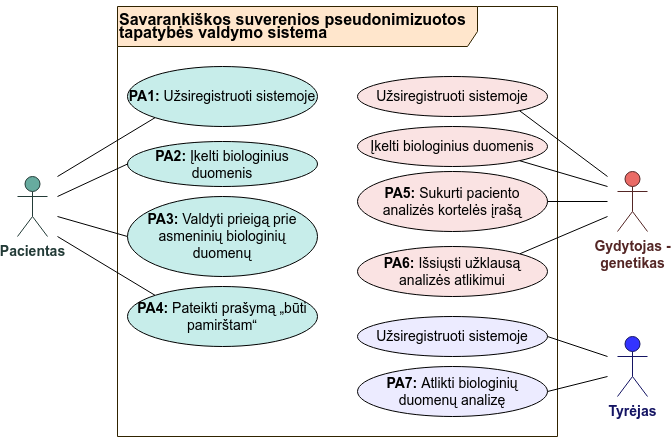
\includegraphics[width=1.05\linewidth]{PAM.png}
        \vspace{-1\baselineskip}
        \caption{\small\textbf{Panaudojimo atvejų modelis (PAM).}}
        \label{fig:image2}
    \end{center}
\end{figure}

\subsection{Panaudojimo atvejų sąrašas}
Žemiau yra pateiktas panaudojimo atvejų sąrašas, kuris turi būti realizuotas
savarankiškos suverenios pseudonimizuotos tapatybės valdymo sistemoje.

\begin{enumerate}[itemsep=0.5pt]
    \item[\textbf{PA1:}] \hyperlink{FR1}{\hypertarget{PA1}{Užsiregistruoti
    sistemoje skirtingų kategorijų naudotojams (pacientams, gydytojams -
    genetikams, tyrėjams).}}
    \item[\textbf{PA2:}] \hyperlink{FR2}{\hypertarget{PA2}{Įkelti biologinius
    duomenis.}}
    \item[\textbf{PA3:}] \hyperlink{FR3}{\hypertarget{PA3}{Valdyti prieigą prie
    asmeninių biologinių duomenų.}}
    \item[\textbf{PA4:}] \hyperlink{FR4}{\hypertarget{PA4}{Pateikti prašymą
    „būti pamirštam“.}}
    \item[\textbf{PA5:}] \hyperlink{FR5}{\hypertarget{PA5}{Sukurti paciento
    analizės kortelės įrašą.}}
    \item[\textbf{PA6:}] \hyperlink{FR6}{\hypertarget{PA6}{Išsiųsti užklausą
    analizės atlikimui.}}
    \item[\textbf{PA7:}] \hyperlink{FR7}{\hypertarget{PA7}{Atlikti biologinių
    duomenų analizę.}}
\end{enumerate}
% \hyperlink{PA5}{item PA1} Taip yra kuriama nuoroda į konkretų PA.
\newpage

\section{Funkciniai reikalavimai ir reikalavimai duomenims}
\subsection{Funkciniai reikalavimai}

\noindent \hypertarget{FR1}{\hyperlink{PA1}{\textbf{PA1:} Užsiregistruoti
sistemoje skirtingų kategorijų naudotojams.}}
\label{sec:FR1}
\begin{table}[htb!]
    \captionsetup{justification=centering}
    \begin{tabular}{|m{3cm}|m{13.7cm}|}
        \hline
        \raggedleft \textbf{\cellcolor{deepchampagne}Tikslas/ uždavinys} &
        Valdyti asmeninius duomenimis ir naudotis sistemoje realizuotu
        funkcionalumu, priklausomai nuo naudotojo kategorijos. \\
        \hline
        \raggedleft \textbf{\cellcolor{deepchampagne}Aprašymas} &
        Realizavus šį panaudojimo atvejį skirtingos naudotojų grupės sistemoje
        gali atlikti skirtingus veiksmus: pacientai gali įkelti savo biologinius
        duomenis ir valdyti kitų asmenų prieigą prie šių duomenų; gydytojai -
        genetikai gali kurti pacientų analizių korteles, bet ir įkelti pacientų
        biologinius duomenis, teikti užklausas tyrėjams dėl biologinių duomenų
        analizės atlikimo, peržiūrėti analizių atlikimo statusą; tyrėjai gali
        vykdyti biologinių duomenų analizes ir teikti jų rezultatus gydytojams -
        genetikams. \\
        \hline
        \raggedleft \textbf{\cellcolor{deepchampagne}Prioritetas} & Aukštas. \\
        \hline
        \raggedleft \textbf{\cellcolor{deepchampagne}Užsakovo (ne)tenkinimas} &
        Netenkinimas: 5, tenkinimas: 5. \\
        \hline
        \raggedleft \textbf{\cellcolor{deepchampagne}Aktorius} &
        Pacientas, gydytojas - genetikas, tyrėjas. \\
        \hline
        \raggedleft \textbf{\cellcolor{deepchampagne}Prieš - sąlyga} &
        Sistemos naudotojas turi būti atsidaręs pradinį sistemos langą. \\
        \hline
        \raggedleft \textbf{\cellcolor{deepchampagne}Sužadinimo sąlyga} &
        Sistemos naudotojas atsidaro sistemos langą, kuriame pateikta
        asmeninės paskyros kūrimo - registracijos - forma. \\
        \hline
        \raggedleft \textbf{\cellcolor{deepchampagne}Pagrindinis
        scenarijus\footnote{Čia ir toliau \textcolor{dartmouthgreen}{žalia}
        spalva pažymėti naudotojo veiksmai.}} & \vskip 5pt
        \makecell[l]{\parbox[t]{13.7cm}{
            \textbf{1.} \textcolor{dartmouthgreen}{Naudotojas užpildo pateiktos
            asmeninės paskyros kūrimo formos laukus.} \\
            \textbf{2.} \textcolor{dartmouthgreen}{Naudotojas išsaugo įvestą
            informaciją, paspausdamas išsaugojimo mygtuką.} \\
            \textbf{3.} {Parodomas informacinis
            pranešimas, informuojantis apie sėkmingai sukurtą asmeninę
            paskyrą.} \\
            \textbf{4.} {Sistema prijungia naudotoją
            prie jo asmeninės paskyros.} \\
            \textbf{5.} {Sistema atidaro naudotojo
            asmeninės paskyros langą.} \\
            \textbf{6. Baigiamas PA.}
        }}
        \\
        \hline
        \raggedleft \textbf{\cellcolor{deepchampagne}Po - sąlyga} &
        Duomenų bazėje sukuriamas naujas sistemos naudotojas, galintis
        prisijungti prie sistemos ir, pagal naudotojo kategoriją, naudotis
        sistemos funkcionalumu. \\
        \hline
        \raggedleft \textbf{\cellcolor{deepchampagne}Alternatyvūs scenarijai} &
        \vskip 5pt
        \makecell[l]{\parbox[t]{13.7cm}{
            \textbf{1.} \textcolor{dartmouthgreen}{Naudotojas užpildo pateiktos
            asmeninės paskyros kūrimo formos laukus.} \\
            \textbf{2.} \textcolor{dartmouthgreen}{Naudotojas išsaugo įvestą
            informaciją, paspausdamas išsaugojimo mygtuką.} \\
            \textbf{3.} Parodomas informacinis pranešimas, informuojantis, kad
            neužpildyti visi privalomi asmeninės paskyros kūrimo formos
            laukai. \\
            \textbf{4.} {Sistema prijungia naudotoją prie jo asmeninės
            paskyros.} \\
            \textbf{5.} {Sistema atidaro naudotojo asmeninės paskyros langą.} \\
            \textbf{6. Baigiamas PA.}
        }}
        \\
        \hline
    \end{tabular}
\end{table}

\newpage

\noindent \hypertarget{FR2}{\hyperlink{PA2}{\textbf{PA2:} Įkelti biologinius
duomenis.}}
\label{sec:FR2}
\begin{table}[htb!]
    \captionsetup{justification=centering}
    \begin{tabular}{|m{3cm}|m{13.7cm}|}
        \hline
        \raggedleft \textbf{\cellcolor{deepchampagne}Tikslas/ uždavinys} &
        Pateikti biologinius duomenis, kurie gali būti panaudoti, siekiant
        išsiaiškinti ligų priežastis, arba moksliniais tikslais. \\
        \hline
        \raggedleft \textbf{\cellcolor{deepchampagne}Aprašymas} &
        Realizavus šį panaudojimo atvejį skirtingos naudotojų grupės sistemoje
        gali atlikti tą patį veiksmą, turint skirtingų siekių: pacientai gali
        įkelti savo biologinius duomenis, kurie gali būti panaudoti moksliniais
        tikslais, papildant biologinių duomenų saugyklą naujais genetiniais
        variantais; gydytojai - genetikai gali įkelti genetinius pacientų
        duomenis, kad jie būtų detaliau išanalizuoti tyrėjų ir būtų galima
        paskirti tolimesnes sutrikimo ar ligos gydymo priemones. \\
        \hline
        \raggedleft \textbf{\cellcolor{deepchampagne}Prioritetas} & Aukštas. \\
        \hline
        \raggedleft \textbf{\cellcolor{deepchampagne}Užsakovo (ne)tenkinimas} &
        Netenkinimas: 5, tenkinimas: 5. \\
        \hline
        \raggedleft \textbf{\cellcolor{deepchampagne}Aktorius} &
        Pacientas, gydytojas - genetikas. \\
        \hline
        \raggedleft \textbf{\cellcolor{deepchampagne}Prieš - sąlyga} &
        Sistemos naudotojas turi būti prisijungęs prie sistemos. \\
        \hline
        \raggedleft \textbf{\cellcolor{deepchampagne}Sužadinimo sąlyga} &
        Sistemos naudotojas atsidaro sistemos langą, kuriame pateikta
        biologinių duomenų įkėlimo skiltis su metaduomenų įvedimo forma. \\
        \hline
        \raggedleft \textbf{\cellcolor{deepchampagne}Pagrindinis
        scenarijus} & \vskip 5pt
        \makecell[l]{\parbox[t]{13.7cm}{
            \textbf{1.} \textcolor{dartmouthgreen}{Naudotojas užpildo pateiktos
            duomenų įkėlimo formos laukus ir prideda biologinius duomenis
            saugantį failą.} \\
            \textbf{2.} \textcolor{dartmouthgreen}{Naudotojas išsaugo įvestą
            metainformaciją bei pridėtą failą, paspausdamas išsaugojimo
            mygtuką.} \\
            \textbf{3.} {Sistema validuoja failo formatą
            ir turinį.} \\
            \textbf{4.} {Sistema užšifruoja duomenis ir
            išsaugo juos duomenų bazėje.} \\
            \textbf{5.} {Sistema įrašo metainformaciją
            apie įkeltą failą į blokų grandinę (taip užtikrinant duomenų
            nekintamumą ir veiksmų atsekamumą).} \\
            \textbf{6.} {Sistema priskiria įrašui
            identifikatorių ir susieja jį su naudotojo paskyra.} \\
            \textbf{7.} {Parodomas informacinis
            pranešimas, informuojantis apie sėkmingai įkeltus duomenis.} \\
            \textbf{8.} \textcolor{dartmouthgreen}{Naudotojas peržiūri įkeltų
            duomenų įrašą savo paskyros skiltyje.} \\
            \textbf{9. Baigiamas PA.}
        }}
        \\
        \hline
        \raggedleft \textbf{\cellcolor{deepchampagne}Po - sąlyga} &
        Į duomenų bazę įkeliami užšifruoti biologiniai duomenys. \\
        \hline
        \raggedleft \textbf{\cellcolor{deepchampagne}Alternatyvūs scenarijai} &
        \vskip 5pt
        \makecell[l]{\parbox[t]{13.7cm}{
            \textbf{1.} \textcolor{dartmouthgreen}{Naudotojas užpildo pateiktos
            duomenų įkėlimo formos laukus ir prideda biologinius duomenis
            saugantį failą.} \\
            \textbf{2.} \textcolor{dartmouthgreen}{Naudotojas išsaugo įvestą
            metainformaciją bei pridėtą failą, paspausdamas išsaugojimo
            mygtuką.} \\
            \textbf{3.} {Sistema validuoja failo formatą
            ir turinį.} \\
            \textbf{4.} {Sistema nesėkmingai užšifruoja
            įkeltą failą dėl vidinės klaidos.} \\
            \textbf{5.} {Parodomas informacinis
            pranešimas, informuojantis, kad duomenų įkėlimas buvo
            nesėkmingas.} \\
            \textbf{6.} {Naudotojui pasiūloma pakartoti
            duomenų įkėlimo veiksmą.} \\
            \textbf{7. Baigiamas PA.}
        }}
        \\
        \hline
    \end{tabular}
\end{table}

\newpage

\noindent \hypertarget{FR3}{\hyperlink{PA3}{\textbf{PA3:} Valdyti prieigą prie
asmeninių biologinių duomenų.}}
\label{sec:FR3}
\begin{table}[htb!]
    \captionsetup{justification=centering}
    \begin{tabular}{|m{3cm}|m{13.7cm}|}
        \hline
        \raggedleft \textbf{\cellcolor{deepchampagne}Tikslas/ uždavinys} &
        Suteikti galimybę naudotojui (pacientui) nuspręsti, ar jo pateikti
        asmeniniai biologiniai duomenys gali būti prieinami kitiems
        naudotojams (gydytojams - genetikams ir tyrėjams). Prieigą prie
        asmeninių biologinių duomenų valdantis asmuo gali suteikti prieigą arba
        atmesti užklausą dėl duomenų prieigos. \\
        \hline
        \raggedleft \textbf{\cellcolor{deepchampagne}Aprašymas} &
        Realizavus šį panaudojimo atvejį skirtingos naudotojų grupės
        (gydytojai - genetikai, tyrėjai) gali vykdyti analizes su pateiktais
        biologiniais duomenimis bei daryti išvadas apie paciento sveikatos
        būklę. Jeigu gydytojai - genetikai arba tyrėjai netenka prieigos
        prie pacientų biologinių duomenų, tolimesnė duomenų analizė yra
        negalima. \\
        \hline
        \raggedleft \textbf{\cellcolor{deepchampagne}Prioritetas} & Aukštas. \\
        \hline
        \raggedleft \textbf{\cellcolor{deepchampagne}Užsakovo (ne)tenkinimas} &
        Netenkinimas: 5, tenkinimas: 5. \\
        \hline
        \raggedleft \textbf{\cellcolor{deepchampagne}Aktorius} &
        Pacientas. \\
        \hline
        \raggedleft \textbf{\cellcolor{deepchampagne}Prieš - sąlyga} &
        Sistemos naudotojas turi būti prisijungęs prie sistemos. \\
        \hline
        \raggedleft \textbf{\cellcolor{deepchampagne}Sužadinimo sąlyga} &
        Sistemos naudotojas atsidaro sistemos langą, kuriame realizuotas duomenų
        prieigos valdymo funkcionalumas. \\
        \hline
        \raggedleft \textbf{\cellcolor{deepchampagne}Pagrindinis
        scenarijus} & \vskip 5pt
        \makecell[l]{\parbox[t]{13.7cm}{
            \textbf{1.} {Sistema pateikia paciento
            įkeltų biologinių duomenų sąrašą.} \\
            \textbf{2.} \textcolor{dartmouthgreen}{Naudotojas pasirenka
            konkretų biologinių duomenų sąrašo įrašą.} \\
            \textbf{3.} {Sistema pateikia naudotojų,
            turinčių prieigą prie konkrečių biologinių duomenų, sąrašą.} \\
            \textbf{4.} \textcolor{dartmouthgreen}{Naudotojas redaguoja
            suteiktas prieigos teises sistemos naudotojams: pratęsia prieigos
            laikotarpį arba atšaukia prieigą.} \\
            \textbf{5.} \textcolor{dartmouthgreen}{Naudotojas suteikia
            naujas prieigas naujiems sistemos naudotojams.} \\
            \textbf{6.} {Sistema atnaujina naudotojams
            suteiktų prieigų sąrašą.} \\
            \textbf{7.} {Sistema įrašo pakeitimo
            informaciją į blokų grandinę.} \\
            \textbf{8.} {Parodomas informacinis
            pranešimas, informuojantis apie sėkmingai atliktą atnaujinimą.} \\
            \textbf{9.} {Sistema informuoja atitinkamus
            sistemos naudotojus apie prieigos teisių pasikeitimus.} \\
            \textbf{10. Baigiamas PA.}
        }}
        \\
        \hline
        \raggedleft \textbf{\cellcolor{deepchampagne}Po - sąlyga} &
        Sistemos naudotojams (gydytojams - genetikams, tyrėjams) yra suteikiama
        arba apribojama prieiga prie paciento biologinių duomenų. \\
        \hline
        \raggedleft \textbf{\cellcolor{deepchampagne}Alternatyvūs scenarijai} &
        \vskip 5pt
        \makecell[l]{\parbox[t]{13.7cm}{
            \textbf{1.} {Sistema pateikia paciento
            įkeltų biologinių duomenų sąrašą.} \\
            \textbf{2.} \textcolor{dartmouthgreen}{Naudotojas pasirenka
            konkretų biologinių duomenų sąrašo įrašą.} \\
            \textbf{3.} {Sistema pateikia naudotojų,
            turinčių prieigą prie konkrečių biologinių duomenų, sąrašą.} \\
            \textbf{4.} \textcolor{dartmouthgreen}{Naudotojas bando redaguoti
            suteiktas prieigos teises konkrečiam naudotojui.} \\
            \textbf{5.} \textcolor{dartmouthgreen}{Parodomas informacinis
            pranešimas, iformuojantis apie nesėkmingą prieigos teisių
            atnaujinimą (tuo atveju, jei naudotojas neaktyvus - nebedirba
            įstaigoje, dirbančioje su kuriama sistema).} \\
            \textbf{6. Baigiamas PA.}
        }}
        \\
        \hline
    \end{tabular}
\end{table}

\newpage

\noindent \hypertarget{FR4}{\hyperlink{PA4}{\textbf{PA4:} Pateikti prašymą
„būti pamirštam“.}}
\label{sec:FR4}
\begin{table}[htb!]
    \captionsetup{justification=centering}
    \begin{tabular}{|m{3cm}|m{13.7cm}|}
        \hline
        \raggedleft \textbf{\cellcolor{deepchampagne}Tikslas/ uždavinys} &
        Leisti naudotojui (pacientui) pateikti prašymą dėl asmeninių ir įkeltų
        biologinių duomenų bei visų su jais susijusių įrašų panaikinimo iš
        saugyklų. \\
        \hline
        \raggedleft \textbf{\cellcolor{deepchampagne}Aprašymas} &
        Remiantis 17 BDAR straipsniu naudotojas turi galėti pateikti prašymą
        ištrinti visus jo pateiktus duomenis. Realizavus šį panaudojimo atvejį
        naudotojui iniciavus duomenų panaikinimą iš duomenų bazių yra ištrinami
        visi saugomi su pacientu susiję biologiniai duomenys bei su jais susiję
        įrašai. \\
        \hline
        \raggedleft \textbf{\cellcolor{deepchampagne}Prioritetas} & Aukštas. \\
        \hline
        \raggedleft \textbf{\cellcolor{deepchampagne}Užsakovo (ne)tenkinimas} &
        Netenkinimas: 3, tenkinimas: 5. \\
        \hline
        \raggedleft \textbf{\cellcolor{deepchampagne}Aktorius} &
        Pacientas. \\
        \hline
        \raggedleft \textbf{\cellcolor{deepchampagne}Prieš - sąlyga} &
        Sistemos naudotojas turi būti prisijungęs prie sistemos. \\
        \hline
        \raggedleft \textbf{\cellcolor{deepchampagne}Sužadinimo sąlyga} &
        Sistemos naudotojas atsidaro asmeninės paskyros peržiūros ir redagavimo
        sistemos langą. \\
        \hline
        \raggedleft \textbf{\cellcolor{deepchampagne}Pagrindinis
        scenarijus} & \vskip 5pt
        \makecell[l]{\parbox[t]{13.7cm}{
            \textbf{1.} \textcolor{dartmouthgreen}{Naudotojas asmeninės paskyros
            redagavimo lange pažymi parinktį „Prašymas būti pamirštam“.} \\
            \textbf{2.} {Sistema pateikia pasekmių,
            susijusių su prašymo būti pamirštam išsiuntimu, sąrašą ir
            nurodo, kad reikalingas naudotojo patvirtinimas.} \\
            \textbf{3.} \textcolor{dartmouthgreen}{Naudotojas patvirtina, kad
            susipažino su pasekmėmis ir patvirtina prašymą.} \\
            \textbf{4.} {Sistema patikrina, ar
            einamuoju metu nėra atliekama paciento pateiktų biologinių duomenų
            analizė.} \\
            \textbf{5.} {Sistema panaikina naudotojo
            asmeninius duomenis, panaikina visų naudotojų prieigas prie
            biologinių duomenų, ištrina visus su naudotoju susijusius duomenis
            iš duomenų bazių ir užfiksuoja „pamiršimo“ įvykį blokų
            grandinėje.} \\
            \textbf{6.} {Parodomas informacinis
            pranešimas, informuojantis apie sėkmingai įgyvendintą prašymą būti
            pamirštam.} \\
            \textbf{7. Baigiamas PA.}
        }}
        \\
        \hline
        \raggedleft \textbf{\cellcolor{deepchampagne}Po - sąlyga} &
        Naudotojo duomenys yra pašalinti, biologiniai duomenys yra nebeprieinami
        kitiems sistemos naudotojams. \\
        \hline
        \raggedleft \textbf{\cellcolor{deepchampagne}Alternatyvūs scenarijai} &
        \vskip 5pt
        \makecell[l]{\parbox[t]{13.7cm}{
            \textbf{1.} \textcolor{dartmouthgreen}{Naudotojas asmeninės paskyros
            redagavimo lange pažymi parinktį „Prašymas būti pamirštam“.} \\
            \textbf{2.} {Sistema pateikia pasekmių,
            susijusių su prašymo būti pamirštam išsiuntimu, sąrašą ir
            nurodo, kad reikalingas naudotojo patvirtinimas.} \\
            \textbf{3.} \textcolor{dartmouthgreen}{Naudotojas patvirtina, kad
            susipažino su pasekmėmis ir patvirtina prašymą.} \\
            \textbf{4.} {Sistema patikrina, ar
            einamuoju metu nėra atliekama paciento pateiktų biologinių duomenų
            analizė.} \\
            \textbf{5.} {Sistema nustato, kad su
            biologiniais duomenimis tebėra atliekami tyrimai.} \\
            \textbf{6.} {Parodomas informacinis
            pranešimas, informuojantis apie einamuoju metu negalimą prašymo
            būti pamirštam įgyvendinimą.} \\
            \textbf{7. Baigiamas PA.}
        }}
        \\
        \hline
    \end{tabular}
\end{table}

\newpage

\noindent \hypertarget{FR5}{\hyperlink{PA5}{\textbf{PA5:} Sukurti paciento
analizės kortelės įrašą.}}
\label{sec:FR5}
\begin{table}[htb!]
    \captionsetup{justification=centering}
    \begin{tabular}{|m{3cm}|m{13.7cm}|}
        \hline
        \raggedleft \textbf{\cellcolor{deepchampagne}Tikslas/ uždavinys} &
        Leisti gydytojui - genetikui sukurti naują paciento kortelės įrašą su
        informacija apie analize.\\
        \hline
        \raggedleft \textbf{\cellcolor{deepchampagne}Aprašymas} &
        Realizavus šį panaudojimo atvejį yra sukuriamas paciento medicininės
        kortelės įrašas, kuriame, esant poreikiui, užfiksuojami paciento
        biologiniai duomenys, pateikiami preliminarūs klinikiniai duomenys,
        aprašoma reikalinga analizė ir įrašomi analizės rezultatai. \\
        \hline
        \raggedleft \textbf{\cellcolor{deepchampagne}Prioritetas} & Aukštas. \\
        \hline
        \raggedleft \textbf{\cellcolor{deepchampagne}Užsakovo (ne)tenkinimas} &
        Netenkinimas: 5, tenkinimas: 5. \\
        \hline
        \raggedleft \textbf{\cellcolor{deepchampagne}Aktorius} &
        Gydytojas - genetikas. \\
        \hline
        \raggedleft \textbf{\cellcolor{deepchampagne}Prieš - sąlyga} &
        Sistemos naudotojas turi būti prisijungęs prie sistemos. \\
        \hline
        \raggedleft \textbf{\cellcolor{deepchampagne}Sužadinimo sąlyga} &
        Sistemos naudotojas atsidaro paciento kortelės įrašų kūrimo langą. \\
        \hline
        \raggedleft \textbf{\cellcolor{deepchampagne}Pagrindinis
        scenarijus} & \vskip 5pt
        \makecell[l]{\parbox[t]{13.7cm}{
            \textbf{1.} \textcolor{dartmouthgreen}{Naudotojas užpildo kortelės
            įrašo formos laukus.} \\
            \textbf{2.} \textcolor{dartmouthgreen}{Naudotojas išsaugo įvestus
            duomenis, paspausdamas išsaugojimo mygtuką.} \\
            \textbf{3.} Parodomas informacinis pranešimas, informuojantis apie
            sėkmingai sukurtą paciento kortelės įrašą. \\
            \textbf{4. Baigiamas PA.}
        }}
        \\
        \hline
        \raggedleft \textbf{\cellcolor{deepchampagne}Po - sąlyga} &
        Analizės užklausa yra užregistruota ir sėkmingai perduota tyrėjo
        vykdymui. \\
        \hline
        \raggedleft \textbf{\cellcolor{deepchampagne}Alternatyvūs scenarijai} &
        \vskip 5pt
        \makecell[l]{\parbox[t]{13.7cm}{
            \textbf{1.} \textcolor{dartmouthgreen}{Naudotojas užpildo kortelės
            įrašo formos laukus.} \\
            \textbf{2.} \textcolor{dartmouthgreen}{Naudotojas išsaugo įvestus
            duomenis, paspausdamas išsaugojimo mygtuką.} \\
            \textbf{3.} Parodomas informacinis pranešimas, informuojantis, kad
            neužpildyti visi privalomi kortelės įrašo kūrimo formos laukai. \\
            \textbf{4. Baigiamas PA.}
        }}
        \\
        \hline
    \end{tabular}
\end{table}

\newpage

\noindent \hypertarget{FR6}{\hyperlink{PA6}{\textbf{PA6:} Išsiųsti užklausą
analizės atlikimui.}}
\label{sec:FR6}
\begin{table}[htb!]
    \captionsetup{justification=centering}
    \begin{tabular}{|m{3cm}|m{13.7cm}|}
        \hline
        \raggedleft \textbf{\cellcolor{deepchampagne}Tikslas/ uždavinys} &
        Leisti gydytojui - genetikui pateikti prašymą tyrėjui atlikti paciento
        biologinių duomenų analizę. \\
        \hline
        \raggedleft \textbf{\cellcolor{deepchampagne}Aprašymas} &
        Realizavus šį panaudojimo atvejį yra išsiunčiamas prašymas biologinių
        duomenų savininkui, kad patvirtintų, ar jis sutinka, kad jo
        biologiniai duomenys būtų analizuojami tyrėjo. Gavus paciento leidimą
        yra informuojamas tyrėjas, kad reikalingas biologinių duomenų analizės
        atlikimas. \\
        \hline
        \raggedleft \textbf{\cellcolor{deepchampagne}Prioritetas} & Aukštas. \\
        \hline
        \raggedleft \textbf{\cellcolor{deepchampagne}Užsakovo (ne)tenkinimas} &
        Netenkinimas: 5, tenkinimas: 5. \\
        \hline
        \raggedleft \textbf{\cellcolor{deepchampagne}Aktorius} &
        Gydytojas - genetikas. \\
        \hline
        \raggedleft \textbf{\cellcolor{deepchampagne}Prieš - sąlyga} &
        Sistemos naudotojas turi būti prisijungęs prie sistemos. \\
        \hline
        \raggedleft \textbf{\cellcolor{deepchampagne}Sužadinimo sąlyga} &
        Sistemos naudotojas atsidaro paciento kortelės įrašų kūrimo langą. \\
        \hline
        \raggedleft \textbf{\cellcolor{deepchampagne}Pagrindinis
        scenarijus} & \vskip 5pt
        \makecell[l]{\parbox[t]{13.7cm}{
            \textbf{1.} \textcolor{dartmouthgreen}{Naudotojas pasirenka analizės
            pateikimo užklausos funkciją.} \\
            \textbf{2.} {Sistema pateikia paciento
            biologinių duomenų, kuriuos galima analizuoti sąrašą.} \\
            \textbf{3.} \textcolor{dartmouthgreen}{Naudotojas pasirenka
            aktualius biologinius duomenis bei įveda kitą su analize susijusią
            informaciją.} \\
            \textbf{4.} {Sistema pateikia tyrėjų, kurie
            gali atlikti analizę, sąrašą.} \\
            \textbf{5.} \textcolor{dartmouthgreen}{Naudotojas pasirenka tyrėją ir
            išsiunčia užklausą pasirinktam tyrėjui.} \\
            \textbf{6.} {Sistema patikrina, ar gydytojas
            ir pasirinktas tyrėjas turi prieigą prie paciento duomenų.} \\
            \textbf{7.} {Sistema užšifruoja užklausą,
            išsaugo ją duomenų bazėje ir išsiunčia parinktam tyrėjui.} \\
            \textbf{8.} {Parodomas informacinis
            pranešimas, informuojantis apie sėkmingai išsiųstą užklausą.} \\
            \textbf{9.} \textcolor{dartmouthgreen}{Naudotojas gali stebėti
            analizės atlikimo būseną.} \\
            \textbf{10. Baigiamas PA.}
        }}
        \\
        \hline
        \raggedleft \textbf{\cellcolor{deepchampagne}Po - sąlyga} &
        Analizės užklausa yra užregistruota ir sėkmingai perduota tyrėjo
        vykdymui. \\
        \hline
        \raggedleft \textbf{\cellcolor{deepchampagne}Alternatyvūs scenarijai} &
        \vskip 5pt
        \makecell[l]{\parbox[t]{13.7cm}{
            \textbf{1.} \textcolor{dartmouthgreen}{Naudotojas pasirenka analizės
            pateikimo užklausos funkciją.} \\
            \textbf{2.} {Sistema pateikia paciento
            biologinių duomenų, kuriuos galima analizuoti sąrašą.} \\
            \textbf{3.} \textcolor{dartmouthgreen}{Naudotojas pasirenka
            aktualius biologinius duomenis bei įveda kitą su analize susijusią
            informaciją.} \\
            \textbf{4.} {Sistema pateikia tyrėjų, kurie
            gali atlikti analizę, sąrašą.} \\
            \textbf{5.} \textcolor{dartmouthgreen}{Naudotojas pasirenka tyrėją
            ir išsiunčia užklausą pasirinktam tyrėjui.} \\
            \textbf{6.} {Sistema patikrina, ar gydytojas
            ir pasirinktas tyrėjas turi prieigą prie paciento duomenų.} \\
            \textbf{7.} {Parodomas informacinis
            pranešimas, informuojantis apie negalimą užklausos išsiuntimą dėl
            duomenų prieigos teisių neturėjimo.} \\
            \textbf{8. Baigiamas PA.}
        }}
        \\
        \hline
    \end{tabular}
\end{table}

\newpage

\noindent \hypertarget{FR7}{\hyperlink{PA7}{\textbf{PA7:} Atlikti biologinių
duomenų analizę.}}
\label{sec:FR7}
\begin{table}[htb!]
    \captionsetup{justification=centering}
    \begin{tabular}{|m{3cm}|m{13.7cm}|}
        \hline
        \raggedleft \textbf{\cellcolor{deepchampagne}Tikslas/ uždavinys} &
        Išanalizuoti paciento biologinius duomenis bei pateikti įžvalgas apie
        juos. \\
        \hline
        \raggedleft \textbf{\cellcolor{deepchampagne}Aprašymas} &
        Realizavus šį panaudojimo atvejį yra įgyvendinama gydytojo - genetiko
        tyrėjui pateikta užklausa dėl biologinių duomenų analizės atlikimo. \\
        \hline
        \raggedleft \textbf{\cellcolor{deepchampagne}Prioritetas} & Aukštas. \\
        \hline
        \raggedleft \textbf{\cellcolor{deepchampagne}Užsakovo (ne)tenkinimas} &
        Netenkinimas: 5, tenkinimas: 5. \\
        \hline
        \raggedleft \textbf{\cellcolor{deepchampagne}Aktorius} &
        Tyrėjas. \\
        \hline
        \raggedleft \textbf{\cellcolor{deepchampagne}Prieš - sąlyga} &
        Sistemos naudotojas turi būti prisijungęs prie sistemos. \\
        \hline
        \raggedleft \textbf{\cellcolor{deepchampagne}Sužadinimo sąlyga} &
        Sistemos naudotojas atsidaro gautą analizės atlikimo užklausą. \\
        \hline
        \raggedleft \textbf{\cellcolor{deepchampagne}Pagrindinis
        scenarijus} & \vskip 5pt
        \makecell[l]{\parbox[t]{13.7cm}{
            \textbf{1.} \textcolor{dartmouthgreen}{Naudotojas peržiūri gautus
            pseudonimizuotus ir užšifruotus biologinius duomenis.} \\
            \textbf{2.} \textcolor{dartmouthgreen}{Naudotojas pasirenka tinkamą
            analizės metodą, naudodamasis integruota arba išorine analizės
            vykdymo programine įranga.} \\
            \textbf{3.} \textcolor{dartmouthgreen}{Naudotojas įkelia analizės
            rezultatus į sistemą.} \\
            \textbf{4.} Sistema informuoja gydytoją - genetiką apie gautus
            analizės rezultatus. \\
            \textbf{5.} Sistema įrašo analizės rezultatą konkretaus paciento
            medicininės kortelės įraše. \\
            \textbf{6. Baigiamas PA.}
        }}
        \\
        \hline
        \raggedleft \textbf{\cellcolor{deepchampagne}Po - sąlyga} &
        Analizės užklausa yra užregistruota ir sėkmingai perduota tyrėjo
        vykdymui. \\
        \hline
        \raggedleft \textbf{\cellcolor{deepchampagne}Alternatyvūs scenarijai} &
        \vskip 5pt
        \makecell[l]{\parbox[t]{13.7cm}{
            \textbf{1.} \textcolor{dartmouthgreen}{Naudotojas peržiūri gautus
            pseudonimizuotus ir užšifruotus biologinius duomenis.} \\
            \textbf{2.} \textcolor{dartmouthgreen}{Naudotojas pasirenka tinkamą
            analizės metodą, naudodamasis integruota arba išorine analizės
            vykdymo programine įranga.} \\
            \textbf{3.} \textcolor{dartmouthgreen}{Atliekant analizę paaiškėja,
            kad pateikti biologiniai duomenys yra nepakankami arba netinkami,
            todėl gydytojo - genetiko siųsta analizės atlikimo užklausa yra
            atmetama, pateikiant detalias atmetimo priežastis.} \\
            \textbf{4. Baigiamas PA.}
        }}
        \\
        \hline
    \end{tabular}
\end{table}

\newpage

\subsection{Reikalavimai duomenims}
\subsubsection{Duomenų modelis}

\subsubsection{Duomenų modelio specifikacija}

\noindent \textbf{E1: Esybė - X.} 
\label{sec:E1}
\begin{table}[htb!]
    \captionsetup{justification=centering}
    \caption{\small\textbf{Esybės 'X' specifikacija}}
    \vskip -10pt
    \begin{tabular}{
        |>{\centering\arraybackslash}m{2cm}
        |>{\centering\arraybackslash}m{5cm}
        |>{\centering\arraybackslash}m{9cm}|
    }
        \hline
        \textbf{\cellcolor{deepchampagne}Atributas} &
        \textbf{\cellcolor{deepchampagne}Atributo apibūdinimas} &
        \textbf{\cellcolor{deepchampagne}Galimos reikšmės}  \\
        \hline
        \multicolumn{1}{|>{\raggedright\ttfamily\arraybackslash}m{2cm}|}
            {Pacientai} &
        \multicolumn{1}{>{\raggedright\arraybackslash}m{5cm}|}{Vietoje, kurioje
        yra sistemos svečias, gali būti silpnas arba spartus internetas.} &
        \multicolumn{1}{>{\raggedright\arraybackslash}m{9cm}|}{Vietoje, kurioje
        yra sistemos svečias, gali būti silpnas arba spartus internetas.}\\
        \hline
    \end{tabular}
    \label{table:ER_specifikacija}
\end{table}

\newpage

\section{Reikalavimai sistemos išvaizdai}
Kuriant savarankiškos suverenios pseudonimizuotos tapatybės valdymo sistemą
turi būti laikomąsi šių sistemos išvaizdos reikalavimų:

\subsubsection*{NF1: Sistemos sąsaja turi būti neįkyri.}
\label{sec:NF1}
\begin{table}[htb!]
    \captionsetup{justification=centering}
    \begin{tabular}{|m{4.9cm}|m{11cm}|}
        \hline
        \raggedleft \textbf{\cellcolor{deepchampagne}Pagrindimas} &
        Sisteminiuose languose neturi būti realizuoti iššokantys modaliniai
        langeliai, kuriuose reikia pasirinkti, ar tikrai norima išsaugoti
        įvestus duomenis. \\
        \hline
        \raggedleft \textbf{\cellcolor{deepchampagne}Šaltinis} & Užsakovas. \\
        \hline
        \raggedleft \textbf{\cellcolor{deepchampagne}Atitikimo kriterijus} & 
        Užpildžius duomenų įvedimo formas ir išsaugojus duomenis nepasirodo
        iššokantis modalinis langelis su pranešimu apie reikalingą duomenų
        įvedimo patvirtinimą - duomenys yra išsaugomi be papildomo naudotojo
        veiksmo. \\
        \hline
        \raggedleft \textbf{\cellcolor{deepchampagne}Užsakovo tenkinimas} & 1. \\
        \hline
        \raggedleft \textbf{\cellcolor{deepchampagne}Užsakovo netenkinimas} & 3. \\
        \hline
        \raggedleft \textbf{\cellcolor{deepchampagne}Prioritetas} & Vidutinis. \\
        \hline
        \raggedleft \textbf{\cellcolor{deepchampagne}Konfliktai} & Nėra. \\
        \hline
    \end{tabular}
\end{table}

\subsubsection*{NF2: Sistema turi būti pritaikyta darbui įvairaus amžiaus
žmonėms.}
\label{sec:NF2}
\begin{table}[htb!]
    \captionsetup{justification=centering}
    \begin{tabular}{|m{4.9cm}|m{11cm}|}
        \hline
        \raggedleft \textbf{\cellcolor{deepchampagne}Pagrindimas} &
        Sistema gali naudotis įvairaus amžiaus asmenys (sistemos svečiai,
        registruoti naudotojai: gydytojai - genetikai, tyrėjai), kurie dėl savo
        amžiaus gali turėti regėjimo sutrikimų, todėl sistemoje turi būti galima
        keisti langų mastelį, neišdarkant sistemos langus sudarančių elementų
        išdėstymo ir nepakenkiant naudotojo naudojimo sistema patirčiai. \\
        \hline
        \raggedleft \textbf{\cellcolor{deepchampagne}Šaltinis} & Užsakovas. \\
        \hline
        \raggedleft \textbf{\cellcolor{deepchampagne}Atitikimo kriterijus} & 
        Sistemos naudotojai, pakeitę mastelį, gali ir toliau sėkmingai naudotis
        sistemos funkcionalumu ir matyti sistemos langus sudarančius elementus
        (nesukeliant naudotojų susierzinimo) dėl sistemos gebėjimo prisitaikyti
        prie keičiamo mastelio. \\
        \hline
        \raggedleft \textbf{\cellcolor{deepchampagne}Užsakovo tenkinimas} & 1. \\
        \hline
        \raggedleft \textbf{\cellcolor{deepchampagne}Užsakovo netenkinimas} & 3. \\
        \hline
        \raggedleft \textbf{\cellcolor{deepchampagne}Prioritetas} & Aukštas. \\
        \hline
        \raggedleft \textbf{\cellcolor{deepchampagne}Konfliktai} & Nėra. \\
        \hline
    \end{tabular}
\end{table}

\newpage

\subsubsection*{NF3: Sistema turi būti intuityvi.}
\label{sec:NF3}
\begin{table}[htb!]
    \captionsetup{justification=centering}
    \begin{tabular}{|m{4.9cm}|m{11cm}|}
        \hline
        \raggedleft \textbf{\cellcolor{deepchampagne}Pagrindimas} &
        Sistema gali naudotis įvairaus amžiaus asmenys, turintys nevienodą
        technologinio raštingumo bei išsilavinimo lygį, todėl sistemos languose
        turi būti naudojami nedviprasmiški ir plačiai visuomenės asmenų daliai
        suprantami sistemos meniu juostos pasirinkimų pavadinimai bei turi būti
        panaudota kuo mažiau kompleksinių informacijos pateikimo struktūrų
        (pavyzdžiui, medžio struktūrų). \\
        \hline
        \raggedleft \textbf{\cellcolor{deepchampagne}Šaltinis} & Užsakovas. \\
        \hline
        \raggedleft \textbf{\cellcolor{deepchampagne}Atitikimo kriterijus} & 
        Jeigu įvykdžius visų sistemos naudotojų apklausą praėjus 2 mėn. po
        naujos poliklinikos sistemos eksploatavimo pradžios nesulaukta daugiau
        nei 10\% atsiliepimų dėl sistemos neintuityvumo, nefunkcinis
        reikalavimas įgyvendintas. \\
        \hline
        \raggedleft \textbf{\cellcolor{deepchampagne}Užsakovo tenkinimas} & 1. \\
        \hline
        \raggedleft \textbf{\cellcolor{deepchampagne}Užsakovo netenkinimas} & 4. \\
        \hline
        \raggedleft \textbf{\cellcolor{deepchampagne}Prioritetas} & Aukštas. \\
        \hline
        \raggedleft \textbf{\cellcolor{deepchampagne}Konfliktai} & Nėra. \\
        \hline
    \end{tabular}
\end{table}

\section{Reikalavimai panaudojamumui}
Kuriant savarankiškos suverenios pseudonimizuotos tapatybės valdymo sistemą
turi būti laikomąsi šių panaudojamumo reikalavimų:

\subsubsection*{NF4: Sistema turi būti nesudėtinga naudotis sistemos
naudotojams.}
\label{sec:NF4}
\begin{table}[htb!]
    \captionsetup{justification=centering}
    \begin{tabular}{|m{4.9cm}|m{11cm}|}
        \hline
        \raggedleft \textbf{\cellcolor{deepchampagne}Pagrindimas} &
        Sistema gali naudotis įvairaus amžiaus bei skirtingo išsilavinimo lygio
        asmenys, todėl sistemos naudotojai turi sugebėti tinkamai naudotis
        sistemos funkcionalumais ir užpildyti sistemoje prieinamas formas be
        papildomų mokymų (turi būti pateikiami detalūs funkcionalumų aprašymai;
        pildant sistemos formas turi būti pateikiami aiškūs ir išsamūs
        paaiškinimai, kokia informacija turi būti įvesta kiekviename lauke). \\
        \hline
        \raggedleft \textbf{\cellcolor{deepchampagne}Šaltinis} & Užsakovas. \\
        \hline
        \raggedleft \textbf{\cellcolor{deepchampagne}Atitikimo kriterijus} & 
        Jeigu įvykdžius sistemos naudotojų apklausą praėjus 2 mėn. po naujos
        poliklinikos sistemos eksploatavimo pradžios nesulaukta nei vieno
        atsiliepimo dėl sudėtingo sistemos naudojimo, nefunkcinis reikalavimas
        įgyvendintas. \\
        \hline
        \raggedleft \textbf{\cellcolor{deepchampagne}Užsakovo tenkinimas} & 2. \\
        \hline
        \raggedleft \textbf{\cellcolor{deepchampagne}Užsakovo netenkinimas} & 2. \\
        \hline
        \raggedleft \textbf{\cellcolor{deepchampagne}Prioritetas} & Aukštas. \\
        \hline
        \raggedleft \textbf{\cellcolor{deepchampagne}Konfliktai} & Nėra. \\
        \hline
    \end{tabular}
\end{table}

\subsubsection*{NF5: Turi būti suteikta galimybė visiems sistemos naudotojams
suprasti sistemoje naudojamus terminus.}
\label{sec:NF5}
\begin{table}[htb!]
    \captionsetup{justification=centering}
    \begin{tabular}{|m{4.9cm}|m{11cm}|}
        \hline
        \raggedleft \textbf{\cellcolor{deepchampagne}Pagrindimas} &
        Sistemoje pateikta informacija turi būti parašyta taip, jog būtų
        suprantama ne tik medicininės dalykinės srities ekspertams. Šalia
        kiekvieno naudojamo medicininio termino turi būti pridėta nuoroda,
        nukreipianti į sistemos langą, kuriame pateiktas techninių terminų
        žodynas. \\
        \hline
        \raggedleft \textbf{\cellcolor{deepchampagne}Šaltinis} & Užsakovas. \\
        \hline
        \raggedleft \textbf{\cellcolor{deepchampagne}Atitikimo kriterijus} & 
        Jeigu įvykdžius sistemos naudotojų apklausą praėjus 2 mėn. po naujos
        poliklinikos sistemos eksploatavimo pradžios nesulaukta nei vieno
        atsiliepimo dėl sudėtingo sistemos naudojimo, nefunkcinis reikalavimas
        įgyvendintas. \\
        \hline
        \raggedleft \textbf{\cellcolor{deepchampagne}Užsakovo tenkinimas} & 2. \\
        \hline
        \raggedleft \textbf{\cellcolor{deepchampagne}Užsakovo netenkinimas} & 2. \\
        \hline
        \raggedleft \textbf{\cellcolor{deepchampagne}Prioritetas} & Žemas. \\
        \hline
        \raggedleft \textbf{\cellcolor{deepchampagne}Konfliktai} & Nėra. \\
        \hline
    \end{tabular}
\end{table}

\section{Reikalavimai vykdymo charakteristikoms}
Kuriant savarankiškos suverenios pseudonimizuotos tapatybės valdymo sistemą
turi būti laikomąsi šių vykdymo charakteristikų reikalavimų:

\subsubsection*{NF6: Autentifikacijos (tapatybės patikrinimo) operacija turi
būti įvykdyta per < 1 s.}
\label{sec:NF6}
\begin{table}[htb!]
    \captionsetup{justification=centering}
    \begin{tabular}{|m{4.9cm}|m{11cm}|}
        \hline
        \raggedleft \textbf{\cellcolor{deepchampagne}Pagrindimas} &
        Greitas autentifikacijos procesas suteikia didesnį naudotojų
        pasitikėjimą sistema bei padeda užtikrinti po autentifikacijos sekančių
        operacijų atlikimą numatytu laiku. \\
        \hline
        \raggedleft \textbf{\cellcolor{deepchampagne}Šaltinis} & Užsakovas. \\
        \hline
        \raggedleft \textbf{\cellcolor{deepchampagne}Atitikimo kriterijus} & 
        Jeigu pasinaudojus įrankiu Apache JMeter laiko tarpas (vidutinis atsako
        laikas) nuo naudotojo autentifikacijos pradžios iki patvirtinimo gavimo
        (fiksuojant tapatybės būsenos pasikeitimą) neviršija 1 s, laikoma, kad
        nefunkcinis reikalavimas įgyvendintas. \\
        \hline
        \raggedleft \textbf{\cellcolor{deepchampagne}Užsakovo tenkinimas} & 2. \\
        \hline
        \raggedleft \textbf{\cellcolor{deepchampagne}Užsakovo netenkinimas} & 2. \\
        \hline
        \raggedleft \textbf{\cellcolor{deepchampagne}Prioritetas} & Žemas. \\
        \hline
        \raggedleft \textbf{\cellcolor{deepchampagne}Konfliktai} & Nėra. \\
        \hline
    \end{tabular}
\end{table}

\subsubsection*{NF7: Patikrinimas, ar naudotojas leido pasiekti genetinius
duomenis, turi būti atliekamas per < 500 ms.}
\label{sec:NF7}
\begin{table}[htb!]
    \captionsetup{justification=centering}
    \begin{tabular}{|m{4.9cm}|m{11cm}|}
        \hline
        \raggedleft \textbf{\cellcolor{deepchampagne}Pagrindimas} &
        Sistemoje pateikta informacija turi būti parašyta taip, jog būtų
        suprantama ne tik medicininės dalykinės srities ekspertams. Šalia
        kiekvieno naudojamo medicininio termino turi būti pridėta nuoroda,
        nukreipianti į sistemos langą, kuriame pateiktas techninių terminų
        žodynas. \\
        \hline
        \raggedleft \textbf{\cellcolor{deepchampagne}Šaltinis} & Užsakovas. \\
        \hline
        \raggedleft \textbf{\cellcolor{deepchampagne}Atitikimo kriterijus} & 
        Jeigu įvykdžius sistemos naudotojų apklausą praėjus 2 mėn. po naujos
        poliklinikos sistemos eksploatavimo pradžios nesulaukta nei vieno
        atsiliepimo dėl sudėtingo sistemos naudojimo, nefunkcinis reikalavimas
        įgyvendintas. \\
        \hline
        \raggedleft \textbf{\cellcolor{deepchampagne}Užsakovo tenkinimas} & 2. \\
        \hline
        \raggedleft \textbf{\cellcolor{deepchampagne}Užsakovo netenkinimas} & 2. \\
        \hline
        \raggedleft \textbf{\cellcolor{deepchampagne}Prioritetas} & Žemas. \\
        \hline
        \raggedleft \textbf{\cellcolor{deepchampagne}Konfliktai} & Nėra. \\
        \hline
    \end{tabular}
\end{table}

% \section{Reikalavimai veikimo sąlygoms}

% \section{Reikalavimai sistemos priežiūrai}

\section{Reikalavimai saugumui}

\subsubsection*{NF8: Visi saugomi genetiniai duomenys turi būti šifruojami.}
\label{sec:NF8}
\begin{table}[htb!]
    \captionsetup{justification=centering}
    \begin{tabular}{|m{4.9cm}|m{11cm}|}
        \hline
        \raggedleft \textbf{\cellcolor{deepchampagne}Pagrindimas} &
        .... \\
        \hline
        \raggedleft \textbf{\cellcolor{deepchampagne}Šaltinis} & Užsakovas. \\
        \hline
        \raggedleft \textbf{\cellcolor{deepchampagne}Atitikimo kriterijus} & 
        Jeigu testuojant šifravimą realiuoju laiku, naudojant tinklo
        analizatorius, asmeninių duomenų negalima perskaityti, laikoma, kad
        nefunkcinis reikalavimas įgyvendintas. \\
        \hline
        \raggedleft \textbf{\cellcolor{deepchampagne}Užsakovo tenkinimas} & 2. \\
        \hline
        \raggedleft \textbf{\cellcolor{deepchampagne}Užsakovo netenkinimas} & 2. \\
        \hline
        \raggedleft \textbf{\cellcolor{deepchampagne}Prioritetas} & Žemas. \\
        \hline
        \raggedleft \textbf{\cellcolor{deepchampagne}Konfliktai} & Nėra. \\
        \hline
    \end{tabular}
\end{table}

\newpage

\subsubsection*{NF9: Naudotojų identifikavimo duomenys turi būti atskirti nuo
genetinių duomenų, naudojant pseudonimizaciją ir anonimizaciją.}
\label{sec:NF9}
\begin{table}[htb!]
    \captionsetup{justification=centering}
    \begin{tabular}{|m{4.9cm}|m{11cm}|}
        \hline
        \raggedleft \textbf{\cellcolor{deepchampagne}Pagrindimas} &
        Sistemos pažeidimo atveju turi būti užtikrintas genetinių duomenų,
        galinčių atskleisti ne tik asmens, bet ir jo šeimos narių asmeninę
        informaciją, konfidencialumas, siekiant išvengti teisės pažeidimų. \\
        \hline
        \raggedleft \textbf{\cellcolor{deepchampagne}Šaltinis} & Užsakovas. \\
        \hline
        \raggedleft \textbf{\cellcolor{deepchampagne}Atitikimo kriterijus} & 
        .... \\
        \hline
        \raggedleft \textbf{\cellcolor{deepchampagne}Užsakovo tenkinimas} & 5. \\
        \hline
        \raggedleft \textbf{\cellcolor{deepchampagne}Užsakovo netenkinimas} & 5. \\
        \hline
        \raggedleft \textbf{\cellcolor{deepchampagne}Prioritetas} & Aukštas. \\
        \hline
        \raggedleft \textbf{\cellcolor{deepchampagne}Konfliktai} & Nėra. \\
        \hline
    \end{tabular}
\end{table}

% \section{Kultūriniai-politiniai reikalavimai}

\section{Teisiniai reikalavimai}

\subsubsection*{NF10: Sistemoje turi būti laikomąsi BDAR reikalavimo dėl
pacientų duomenų pseudonimizavimo.}
\label{sec:NF10}
\begin{table}[htb!]
    \captionsetup{justification=centering}
    \begin{tabular}{|m{4.9cm}|m{11cm}|}
        \hline
        \raggedleft \textbf{\cellcolor{deepchampagne}Pagrindimas} &
        Sistemos, kuriose vykdomas asmenų biologinių duomenų saugojimas bei
        apdorojimas, turi atitikti BDAR 32 straipsnyje aprašytą reikalavimą,
        nurodantį, tvarkant asmens duomenis turi būti naudojamos tinkamos
        techninės ir organizacinės priemonės, įskaitant pseudonimizavimą,
        siekiant užtikrinti duomenų saugumą. \\
        \hline
        \raggedleft \textbf{\cellcolor{deepchampagne}Šaltinis} & Užsakovas. \\
        \hline
        \raggedleft \textbf{\cellcolor{deepchampagne}Atitikimo kriterijus} & 
        Laikoma, kad nefunkcinis reikalavimas įgyvendintas, jeigu atlikus
        sistemos duomenų bazės struktūros analizę nenustatomas genetinių duomenų
        saugojimas kartu su identifikavimo duomenimis bei testavimo metu
        nenustatyti tiesiogiai identifikuojantys asmeniniai duomenys. \\
        \hline
        \raggedleft \textbf{\cellcolor{deepchampagne}Užsakovo tenkinimas} & 5. \\
        \hline
        \raggedleft \textbf{\cellcolor{deepchampagne}Užsakovo netenkinimas} & 5. \\
        \hline
        \raggedleft \textbf{\cellcolor{deepchampagne}Prioritetas} & Aukštas. \\
        \hline
        \raggedleft \textbf{\cellcolor{deepchampagne}Konfliktai} & Nėra. \\
        \hline
    \end{tabular}
\end{table}

\newpage

% \section{Egzistuojantys sprendimai (Off-the-Shelf Solutions)}
% \subsection{Pagamintos sistemos, kurios gali būti nupirktos}

% \subsection{Pagaminti komponentai, kurie gali būti panaudoti}

% \subsection{Galimas pakartotinas panaudojimas}

\newpage

\section{Naujos problemos}
\subsection{Problemos diegimo palinkai}

\subsection{Įtaka jau instaliuotoms sistemoms}

\subsection{Neigiamas vartotojų nusiteikimas}

\subsection{Kliudantys diegimo aplinkos apribojimai}

\subsection{Galimos naujos sistemos sukeltos problemos}

\newpage

\section{Uždaviniai}
\subsection{Sistemos pateikimo žingsniai (etapai)}

% 21.1.Sistemos pateikimo žingsniai (etapai)
% Aprašoma sistemos gyvavimo ciklo detalės bei sistemos pateikimo būdas. Tam tikslui gali būti tinkama aukšto lygio (nedetalizuota) procesų diagrama, kurioje parodomi realizuojami uždaviniai bei jų sąsaja. Punktas skirtas numatyti būdus sistemai pateikti, kad kiekvienas turėtų vienodą supratimą apie sistemą. Nereikėtų pamiršti duomenų perkėlimo, apmokymo ir kitų uždavinių.

\subsection{Vystymo etapai}
% 21.2.Vystymo etapai
% Sistemos kiekvienos vystymo fazės (etapo) specifikacija bei veikimo aplinkos komponentų charakterizavimas. Punkto paskirtis - numatyti etapus naujos sistemos veikimo aplinkai sukurti, kad kūrimo procesą būtų galima valdyti. Būtina numatyti techninę bei kitą įrangą , reikalingą kiekviename sistemos kūrimo etape. Tai gali galutinai paaiškėti tik projektavimo etape.

\newpage

\section{Rizikos ir jų valdymas}
\noindent \textbf{R1:} Pakeisti ar sugadinti biologiniai duomenys gali lemti
neteisingą analizę.

\label{sec:R1}
\begin{table}[htb!]
    \captionsetup{justification=centering}
    \vskip -10pt
    \begin{tabular}{|m{3cm}|m{13.7cm}|}
        \hline
        \raggedleft \textbf{\cellcolor{deepchampagne}Valdymas} &
        Biologinius duomenis integruoti į blokų grandinę, siekiant užtikrinti
        duomenų nekintamumą. \\
        \hline
        \raggedleft \textbf{\cellcolor{deepchampagne}Tikimybė} & Žema. \\
        \hline
        \raggedleft \textbf{\cellcolor{deepchampagne}Poveikis} & Aukštas. \\
        \hline
    \end{tabular}
\end{table}

\noindent \textbf{R2:} Nepaisant pseudonimizavimo, biologiniai duomenys gali
būti susieti su konkrečiais asmenimis.

\label{sec:R2}
\begin{table}[htb!]
    \captionsetup{justification=centering}
    \vskip -10pt
    \begin{tabular}{|m{3cm}|m{13.7cm}|}
        \hline
        \raggedleft \textbf{\cellcolor{deepchampagne}Valdymas} &
        Griežtai riboti prieigos teises pagal naudotojo kategoriją ir vykdyti
        duomenų pseudonimų keitimą. \\
        \hline
        \raggedleft \textbf{\cellcolor{deepchampagne}Tikimybė} & Žema. \\
        \hline
        \raggedleft \textbf{\cellcolor{deepchampagne}Poveikis} & Aukštas. \\
        \hline
    \end{tabular}
\end{table}

\noindent \textbf{R3:} Sistemoje realizuotas funkcionalumas gali neatitikti
asmens duomenų apsaugos reikalavimų.

\label{sec:R3}
\begin{table}[htb!]
    \captionsetup{justification=centering}
    \vskip -10pt
    \begin{tabular}{|m{3cm}|m{13.7cm}|}
        \hline
        \raggedleft \textbf{\cellcolor{deepchampagne}Valdymas} &
        Skirti ypatingą dėmesį BDAR reglamento analizei ir atitinkamam sistemos
        pritaikymui. \\
        \hline
        \raggedleft \textbf{\cellcolor{deepchampagne}Tikimybė} & Žema. \\
        \hline
        \raggedleft \textbf{\cellcolor{deepchampagne}Poveikis} & Aukštas. \\
        \hline
    \end{tabular}
\end{table}

\noindent \textbf{R4:} Dėl sistemos gedimo ar neteisingo atsarginio kopijavimo
gali būti prarasti duomenys.

\label{sec:R4}
\begin{table}[htb!]
    \captionsetup{justification=centering}
    \vskip -10pt
    \begin{tabular}{|m{3cm}|m{13.7cm}|}
        \hline
        \raggedleft \textbf{\cellcolor{deepchampagne}Valdymas} &
        Vykdyti reguliarų duomenų atsarginių kopijų kūrimą, aiškiai dokumentuoti
        duomenų atstatymo procesą bei periodiškai vykdyti šio proceso
        testavimą. \\
        \hline
        \raggedleft \textbf{\cellcolor{deepchampagne}Tikimybė} & Žema. \\
        \hline
        \raggedleft \textbf{\cellcolor{deepchampagne}Poveikis} & Aukštas. \\
        \hline
    \end{tabular}
\end{table}

\noindent \textbf{R5:} Sistemos veikimo sutrikimai, galintys kilti po
sistemos diegimo į užsakovo aplinkas.

\label{sec:R5}
\begin{table}[htb!]
    \captionsetup{justification=centering}
    \vskip -10pt
    \begin{tabular}{|m{3cm}|m{13.7cm}|}
        \hline
        \raggedleft \textbf{\cellcolor{deepchampagne}Valdymas} &
        Pradėti vykdyti sistemos testavimą ankstyvosiose sistemos vystymo
        stadijose, siekiant ištestuoti visą sistemos funkcionalumą, bei turėti
        aiškiai dokumentuotą sistemos diegimo planą, kuriame būtų detaliai
        aprašyti ir veiksmai, kurių reikia imtis nesėkmingo diegimo atveju. \\
        \hline
        \raggedleft \textbf{\cellcolor{deepchampagne}Tikimybė} & Aukšta. \\
        \hline
        \raggedleft \textbf{\cellcolor{deepchampagne}Poveikis} & Aukštas. \\
        \hline
    \end{tabular}
\end{table}

\noindent \textbf{R6:} Dėl nenumatytų priežasčių gali vėluoti projektas -
sistema gali būti sudiegta vėliau nei yra numatyta projekto plane.
\label{sec:R6}
\begin{table}[htb!]
    \captionsetup{justification=centering}
    \vskip -10pt
    \begin{tabular}{|m{3cm}|m{13.7cm}|}
        \hline
        \raggedleft \textbf{\cellcolor{deepchampagne}Valdymas} &
        Pradėti vykdyti sistemos testavimą ankstyvosiose sistemos vystymo
        stadijose, siekiant identifikuoti klaidas kuo anksčiau, bei organizuoti
        reguliarius susitikimus su užsakovu, kad būtų aptartas darbų progresas
        bei iškilę sunkumai. \\
        \hline
        \raggedleft \textbf{\cellcolor{deepchampagne}Tikimybė} & Aukštas. \\
        \hline
        \raggedleft \textbf{\cellcolor{deepchampagne}Poveikis} & Aukštas. \\
        \hline
    \end{tabular}
\end{table}

\newpage

\section{Kaina}

\section{Naudotojo dokumentacija}
Žemiau yra pateiktas naudotojams aktualios dokumentacijos aprašymas.

\begin{table}[htb!]
    \captionsetup{justification=centering}
    \begin{tabular}{|m{6cm}|m{10cm}|}
        \hline
        \raggedleft \textbf{\cellcolor{deepchampagne}Pavadinimas} &
        Sistemos naudojimo vadovas. \\
        \hline
        \raggedleft \textbf{\cellcolor{deepchampagne}Atsakingas asmuo} &
        Danielė Stasiūnaitė. \\
        \hline
        \raggedleft \textbf{\cellcolor{deepchampagne}Naudotojų įtraukimas į
        dokumentacijos ruošimą} & 
        Tiesioginių sistemos naudotojų įtraukimas į naudotojo vadovo kūrimą yra
        nenumatytas. \\
        \hline
        \raggedleft \textbf{\cellcolor{deepchampagne}Dokumento atnaujinimas} &
        Jeigu po pagrindinio sistemos diegimo tebėra atliekami reguliarūs
        sistemos vystymo ir tobulinimo darbai, naudojimo vadovas turi būti
        atnaujinamas ir perduodamas užsakovui kas 2 mėnesius. Kitu atveju,
        naudojimo vadovas atnaujinamas tik atskiru užsakovo prašymu. \\
        \hline
        \raggedleft \textbf{\cellcolor{deepchampagne}Dokumento pateikimo forma
        ir turinys} &
        Sistemos naudojimo vadovas turi būti prieinamas pradiniame sistemos
        lange kaip atskiras atsisiunčiamas PDF dokumentas. Vadove turi būti
        pateiktas sistemos pavadinimas, dokumento versija, rengimo data,
        atsakingas asmuo, sistemos paskirtis bei turi būti aprašytos visos
        sistemoje realizuotos funkcijos. \\
        \hline
    \end{tabular}
\end{table}
% 25.Vartotojo dokumentacija ir apmokymas
% Pateikiamas vartotojui reikalingos dokumentacijos sąrašas. Tikslas - įvertinti dokumentacijos poreikį ir numatyti atsakingus asmenis jai parengti. Klausimai, į kuriuos reikia atsakyti:
% •Kokio lygio dokumentacija reikalinga?
% •Ar vartotojai dalyvaus rengiant dokumentaciją?
% •Kas bus atsakingas už savalaikį dokumentacijos rengimą ir atnaujinimą?
% •Kokia dokumentacijos pateikimo forma?

% \section{Perspektyviniai reikalavimai (Waiting room)}
% \section{Idėjos sprendimams (Ideas for solutions)}



% KABUTĖS: „ “
\end{document}



% Reikalavimų specifikacijos paaiškinimai
% (Volere Šablonas)
% Projekto varovai (Project Drivers)
% 1.Sistemos paskirtis
% Tai sistemos kūrimo priežastis bei nauda, kurią sistema duos, jeigu bus sukurta;Čia gali būti įvardintos veiklos problemos, su kuriomis susiduria klientas, numatant, kaip jas gali išspręsti kuriama sistema 
% 1.1. Projekto kūrimo pagrindas (pagrindimas)
% Projekto pagrindimui gali būti pasiremta įvairiomis nuorodomis, argumentuojančiomis sistemos kūrimo reikalingumą. Galimas atvejis, kad problemos nėra, tačiau yra poreikis (galimybė) plėsti tam tikrą veiklą. Tuomet tokia galimybė turi būti aprašyta 
% 1.2. Sistemos tikslai (paskirtis)
% Aprašoma, ko norima iš sistemos, ką ji turi atlikti, kaip ji įtakos veiklos tikslų sėkmingą pasiekimą.
% 2.Užsakovai, pirkėjai ir kiti sistema suinteresuoti asmenys
% Būtina turėti informaciją apie šiuos asmenis, kad išvengti skaudžių netikėtumų.
% 1.Užsakovas. Tai asmuo, kuris apmoka sistemos kūrimo darbus ir taps šios sistemos savininku. dažnai tai asmuo, esantis sistemos vartotojo padalinio vadovu. Šiame punkte nurodomi šio asmens duomenys. Kartais gali būti keli asmenys. Užsakovas priima galutinį produktą (sistemą), todėl turi būti juo patenkintas. Jei sistema kuriama savoms reikmėms, tai užsakovas ir pirkėjas gali būti tas pats asmuo. Jei sistema kuriama rinkai (išorės vartotojams), tuomet užsakovu gali būti marketingo skyrius, kurį atstovauja šio skyriaus darbuotojas
% 2.Pirkėjas. Tai sistemą perkantis asmuo (atstovaujantis organizaciją). Jei sistema skirta savoms reikmėms, tai pirkėjas yra asmuo, kuris priima galutinį sprendimą, ar sistema reikalinga. Tai gali būti padalinio, kuriame diegiama sistema, vadovas, arba visos organizacijos vadovas. Jei sistema skirta rinkai, tai pirkėjas yra sistemą įsigyjančią organizaciją atstovaujantis asmuo. Jei pirkėją atstovauja sistemą platinančios organizacijos marketingo skyrius, tuomet jie turi pateikti kuo tikslesnę numatomų faktinių pirkėjų charakteristiką. 
% 3.Kiti sprendimus priimantys asmenys. Pateikiama informacija apie kitus sistemos kūrimą įtakojančius asmenis. Tai gali būti: 
% Vadovybė arba projekto rėmėjai;
% Veiklos srities ekspertai;
% Techniniai specialistai;
% Projektuotojai;
% Marketingo specialistai;
% Projekto vadovai;
% Testuotojai ir kokybę tikrinantys asmenys;
% Inspektoriai (darbo saugos) arba auditoriai;
% Teisininkai.
% Šie asmenys išreiškia tam tikrus reikalavimus sistemai.

% 3.Vartotojai
% Tai asmenų, kurie betarpiškai naudosis sistema, sąrašas. Kiekvienai vartotojų kategorijai reikia nurodyti tokią informaciją:
% •Vartotojo kategorija, pav., mokinys, inžinierius, projekto vadovas;
% •Vartotojo sprendžiami uždaviniai (atliekamos funkcijos) - tai vartotojo funkcijų suvestinė;
% •Patirtis dalykinėje srityje - naujokas, įprastas darbuotojas, srities specialistas (meistras);
% •Patirtis informacinėse technologijose - naujokas, patyręs, informatikas;
% •Papildomos vartotojo  charakteristikos - turinčios įtaką reikalavimams bei sistemos savybėms. Tai gali būti:
% •fizinės galimybės (negalia);
% •intelektualinės galimybės (negalia);;
% •požiūris į darbą;
% •požiūris į IT;
% •apsimokymo poreikis;
% •kalbos įgūdžiai;
% •amžiaus grupė;
% •lytis.
% Vartotojo charakteristika turi būti įvertinta pildant šablono punktą 4.1. Ji gali labai įtakoti priimamus projektinius sprendimus, nes vartotojai gali būti įvairiausi žmonės, kurių interesai ir charakteristikos labai skirtingos: dvasininkai; atsitiktiniai asmenys; neraštingi asmenys; nuo sistemos “nutolę” asmenys; saugumo tarnybų darbuotojai; žmonės, dirbsiantys per telefoną ar internetą ir t.t.
% •Vartotojų prioritetai. Kiekvienai vartotojų grupei rekomenduojama suteikti prioritetą. Tai gali būti:
% •svarbiausi vartotojai - jų nuomonė ir pageidavimai svarbiausi;
% •antraeiliai vartotojai - jei kyla konfliktas su pirmąja grupe, tai jų nuomonė turi didesnę įtaką;
% •nesvarbūs (atsitiktiniai) vartotojai

% Projekto Apribojimai
% Tai apribojimai, kurie įtakoja reikalavimų specifikaciją bei sistemos kūrimo eigą bei charakteristikas.

% 4.Įpareigojantys apribojimai. (Mandated constraints) 
% 4.1. Apribojimai sprendimui
% Tai išankstiniai apribojimai sistemos kūrimo eigai ar charakteristikoms. Jie turi nurodymo (griežto reikalavimo) pobūdį. Juos reikia tiksliai aprašyti, nepamirštant numatyti, kaip galima “išmatuoti” (testuoti) jų laikymąsi sukurtoje sistemoje. Čia galima apibūdinti ir tokio apribojimo atsiradimo priežastis.
% Šiuos apribojimus dažniausiai pateikia užsakovas, pirkėjas arba vartotojas dėl įvairiausių priežasčių. Neįvertinus šių apribojimų, sistema gali būti nepriimta. Šie apribojimai apibrėžia tam tikrą galimų sprendimų kontekstą, todėl juos reikia registruoti itin kruopščiai. Negalima apriboti laisvės priimti geresnį sprendimą. Čia gali būti pateikiami tik neginčytini apribojimai.

% 4.2.Diegimo aplinka
% Charakterizuojama technologinė ir fizinė aplinka, kurioje sistema bus įdiegta. Tai apima automatizavimo, mechanizavimo, organizacinius ir kitokius įrenginius, kurie atspindi su kuriama sistema bendradarbiausiančias sistemas (nevertinant žmogaus)
% Tai technologinės aplinkos aprašas, kuris leidžia sistemos projektuotojams įvertinti ir realizuoti reikalingas komunikavimo tarp sistemos ir technologinės aplinkos priemones. Šio aprašo pagrindu sudaroma šablono punkto 4.3 specifikacija. Čia pateikiamos diegimo aplinkos visos pagrindinės charakteristikos. Jei sistema įtakos organizacinę struktūrą, tuomet galima įdėti organizacinę schemą (organization chart).

% 4.3.Bendradarbiaujančios sistemos
% Carakterizuojama sisteminė aplinka (posistemės) - su kuria kuriama sistema turės bendradarbiauti. Tai gali būti: kitos taikomosios sistemos (posistemiai), sukurtos išimtinai šiai organizacijai; specializuoti komerciniai programų paketai ir t.t. Šis punktas apibrėžia integravimo uždavinius ir problemas. Patikrinkite veiklos konteksto modelį, kad nustatyti, ar nėra gretimų sistemų, kurias galima įvardinti kaip komunikuojančias sistemas. 

% 4.4.Komerciniai specializuoti programų paketai
% Carakterizuojami specializuoti į kuriamą sistema numatomi įtraukti programų paketai, kurie bus reikalingi kuriamos sistemos funkcionalumui užtikrinti. ai reikalinga įvertinti, kadangi papildomų paketų charakteristikos, sąsajos sudėtis bei “elgesys” turi įtaką formuojant reikalavimus kuriamai sistemai;
% Formuojant reikalavimus gali išryškėti prieštaravimai tarp reikalavimų ir numatomų naudoti specializuotų paketų. Tuomet tenka svarstyti, ar įmanoma tokius prieštaravimus išspręsti, ar specializuotas paketas yra geras sprendimo variantas.

% 4.5.Numatoma darbo vietos aplinka
% Carakterizuojama aplinka, kurioje dirbs sistemos vartotojas. Aprašomos darbo vietos savybės, kurios gali turėti įtakos sistemos projektavimui. Punkto tikslas - fizinės darbo vietos charakteristikų, kurios gali įtakoti reikalavimus sistemai, identifikavimas. Sistema turės kompensuoti darbo vietos keliamus sunkumus ir įvertinti esamus apribojimus. Tai gali būti, pavyzdžiui: “spausdintuvas bus toli nuo vartotojo darbo vietos” - matyt nereikėtų teikti prioriteto spausdintiems sistemos rezultatams; “darbo vieta yra lauke”; “darbo vieta triukšminga “ - garsiniai signalai neduos efekto; “darbo vieta mobili”.

% 4.6.Sistemos kūrimo terminai
% Numatomi visi laiko apribojimai arba galimi terminų keitimo (tikslinimo) faktoriai. Būtina numatyti konkrečias datas ir argumentus, kodėl tokie terminai fiksuojami. Gali būti numatomos ir atskirų sistemos dalių užbaigimo ar parengimo testavimui datos. Gali būti pateikiamos įvairios griežtų terminų priežastys: tenka laikytis numatyto sistemos paleidimo grafiko; kitų veiklos sričių ar sistemų priklausomybė nuo kuriamos sistemos; rinkos tyrimo rezultatų pagrindu (susidaro palanki situacija); veiklos, naudosiančios sistemą, vystymas pagal grafiką. Tikslinga įvertinti terminų nesilaikymo pasekmes (“Kas bus jei…”)

% 4.7.Sistemos kūrimo biudžetas
% Numatomi sistemos kūrimo finansiniai ištekliai kiekine išraiška. Reikalavimai negali viršyti biudžeto, todėl dalies reikalavimų gali tekti atsisakyti. Įvertinus numatomą skirti biudžetą, galima identifikuoti, ar sistema tikrai reikalinga (ar jos tikrai pageidaujama).

% 5.Terminų žodynas
% Pateikiamas terminų, kurie bus naudojami specifikuojant reikalavimus, žodynas. Žodyne sukaupiamos dalykinėje srityje naudojamos standartinės sąvokos. Kiekvienai sąvokai pateikiamas glaustas paaiškinimas. Sąvokos turi būti priimtinos dalykinės srities atstovams. Šio punkto paskirtis - sudaryti dalykinės srities sąvokų žodyną, dėl ko gali būti sutaupyta daug laiko įvairiems paaiškinimams. Taip išvengiama nesusipratimų. Žodynas naudojamas bei papildomas sistemos projektavimo metu

% 6.Svarbūs faktai ir prielaidos
% Išoriniai faktoriai, įtakojantys kuriamą sistemą, tačiau nepriklausantys iš anksto nustatomiems apribojimams, kurie įtakoja reikalavimų specifikaciją. Šiame punkte charakterizuojami kiti išoriniai veiksniai, sistemos, veiklos (pasaulio mastu), galintys įtakoti sistemą. Svarbūs faktai ne visuomet transformuojami į reikalavimus, tačiau toks atvejis galimas. Į šį punktą įtraukiami tie faktai, kurie nepatenka į kitus šablono punktus, tačiau numanoma, kad jie įtakoja reikalavimų specifikaciją

% Pateikiamas prielaidų sąrašas, kurias pateikia sistemos kūrėjai. Jos gali liesti įvairius sistemos kūrimo aspektus. Prielaidos, tam tikra prasme, yra faktų priešingybė, nes gali būti neteisingos, tačiau gali ir pasiteisinti. Šis punktas turi dvi paskirtis: suteikti galimybę pateikti prielaidas; susipažinti su pateiktomis prielaidomis.
% Tai gali būti prielaidos dėl:
% • kitų sistemos dalių, kitų sistemų, programų paketų ar komponentų parengtumo naudojimui, kai to reiks projektuotojui;
% •sistemos veikimo technologinės aplinkos (suderinamumo aspektas);
% •vartotojo galimybių;
% •kitų sistemų, kurios kuriamos kartu su pastarąja sistema;
% •kitų (pirktinių) komponentų panaudojimo galimybių;
% •priklausomybių nuo išorinių sistemų ar asmenų;
% •naujų įstatymų ar politinių sprendimų.


% Funkciniai reikalavimai
% 7.Veiklos sfera (The scope of the work)
% 7.1.Veiklos kontekstas (pateikiama konteksto diagrama)
% Nagrinėjamai veiklos sričiai apibrėžti naudojama “Konteksto diagrama”. Šią sritį tenka ištirti, kad sukurti sistemą. Veiklos kontekstas apima plačiau, nei kuriamos sistemos atliekamos funkcijos. Kol nesuprasime darbo (veiklos), kuriam turi talkinti sistema, tol nesukursime tinkamos sistemos, kurį “įsirašys” į aplinką. Veiklos kontekstas apibrėžia dominančią veiklą ir jos naudojamus bei formuojamus informacijos srautus. Veiklos “atsakomybė” prasideda kai informacijos srautas įeina į sistemą ir baigiasi, kai rezultatinis srautas išeina iš sistemos. Išorinės esybės diagramoje modeliuoja kaimynines (gretimas) sistemas (tai aplinkinės sistemos arba žmonės)

% Konteksto diagrama ( pavyzdys)
% Sąsaja tarp kaimyninių sistemų ir veiklos konteksto nusako, dėl kokių priežasčių kaimyninė sistema mus domina. Informacijos srautai tarp gretimų sistemų ir veiklos srities nusako, už ką yra atsakinga nagrinėjama veikla ir už ką - kaimyninės sistemos

% 7.2.Veiklos padalinimas
% Sudaromas veiklos įvykių sąrašas, kuris apima visus veiklos įvykius, už kuriuos yra atsakinga nagrinėjama veikla. Veiklos įvykiai - tai vartotojo išskiriami veiksmai, atliekami veiklos metu. Reakcija (atsakymas) į kiekvieną įvykį atvaizduoja veiklos dalį, įeinančią į bendras veiklą sudarančias funkcijas.
% Įvykių sąrašą sudaro: 1) Įvykio pavadinimas; 2) Įeinantys ir išeinantys informacijos srautai, kurie “lydi” įvykį. eiklos padalinimo paskirtis - identifikuoti veiklos “gabaliukus” , kurių pagrindu būtų galima nustatyti reikalavimus. iklos įvykių pagrindu toliau galima remtis atliekant  sistemos detalią analizę ir projektavimą.



% Lentelė. Veiklos įvykių sąrašas ( pavyzdys)

% 8.
% Produkto veiklos sfera (The scope of the product)
% 8.1.Sistemos ribos
% Ribas tarp sistemos ir vartotojo nusako panaudojimo atvejų diagrama. Panaudojimo atvejų diagrama sudaroma įvertinant kiekvieną išskirtą veiklos įvykį ir kuriamos sistemos indėlį šio įvykio atžvilgiu




% Panaudojimo atvejų diagrama ( pavyzdys)

% 8.2.Panaudojimo atvejų sąrašas
% Panaudojimo atvejų diagrama apjungia visus sistemos apimamus panaudojimo atvejus. Jei jų skaičius viršija 15-20, tuomet tikslinga sudaryti jų sąrašą ir modeliuoti atskirais fragmentais. Kiekvienam sąrašo panaudojimo atvejui pateikiamas :
% 1) panaudojimo atvejo numeris;
% 2) vartotojo / aktoriaus pavadinimas;
% 3) panaudojimo atvejo aprašas; 
% 4) panaudojimo atvejo tenkinimo kriterijus.
% Jei yra sudarytas panaudojimo atvejo aprašas ir (arba) tam tikri jo scenarijaus modeliai, tuomet panaudojimo atvejų sąraše gali būti nuoroda į šią medžiagą.

% 1. PANAUDOJIMO ATVEJIS: Informacijos apie personalą registravimas

% Vartotojas/Aktorius: 	Laivo vado pavaduotojas
% Aprašas: 	Apima procesą, kurio metu laivo vado pavaduotojas registruoja informaciją apie laivo personalą.
% Prieš sąlyga: 	Asmuo nėra registruotas sistemoje;
% 			Asmuo dalyvaus apskaitos procesuose.
% Sužadinimo sąlyga: 	Atsirado naujas asmuo, kuris bus personalo narys (dalyvaus apskaitoje).
% Po-sąlyga: 	Sistemoje užregistruojamas naujas personalo asmuo.

% Panaudojimo atvejo aprašas (pavyzdys)


% 9.Funkciniai reikalavimai ir reikalavimai duomenims
% Funkcinius ir nefunkcinius reikalavimus tikslinga pateikti prisilaikant vieningos formos. Ši forma atstoja vieningą reikalavimo specifikavimo struktūrą. Ši reikalavimų forma gali būti pateikiama ant atskiros kortelės, tačiau vėliau tokiu pavidalu užregistruota reikalavimų specifikacija gali būti apdorojama kompiuterizuotu būdu. 

% FORMA REIKALAVIMAMS REGISTRUOTI

% Reikalavimo identifikavimas. Reikalavimas identifikuojamas trimis parametrais:
% •numeriu;
% •tipu;
% •įvykiu arba panaudojimo atvejo numeriu.
% Reikalavimas turi būti trasuojamas (stebimas) per visą sistemos kūrimo laiką, todėl logiška, kad numeravimas turi būti unikalus.
% Suklasifikavus reikalavimus pagal tipus paprasčiau:
% • nustatyti, kurie iš jų prieštarauja tarpusavyje;
% • numatyti reikiamą tikimo kriterijų;
% • aptikti dubliavimąsi ir trūkstamus reikalavimus.
% Įvykių numeriai gali būti pritaikyti panaudojimo atvejams numeruoti, tačiau gali būti ir nesutapimų. Reikalavimas susiejamas su panaudojimo atvejais, nurodant jų numerius.
% Aprašymas skirtas reikalavimo paskirčiai apibrėžti. Tai tekstinis reikalavimo apibrėžimas. Jame turi atsispindėti užsakovo arba vartotojo pageidavimai. Geriausia apsiriboti vienu aprašymo sakiniu. 

% Pagrindimas skirtas nusakyti reikalavimo reikalingumą. Jame nurodoma, kodėl reikalavimas svarbus, kokia jo įtaka sistemos tikslams. Pagrindimas atskleidžia reikalavimo prasmę bei įtaką visai sistemai, todėl gali būti panaudotas įvertinant reikalavimo reikalingumą bei kokybę. 

% Šaltinis - tai asmuo, kuris iškėlė reikalavimą. Tradiciškai tai tam tikromis žiniomis (susijusiomis su reikalavimu) pasižymintis ir pareigas užimantis asmuo. 

% Tinkamumo kriterijus - tai kvantifikuotas tikslas, kurį turi tenkinti sistema. Nors reikalavimas aprašomas vartotojo sąvokomis, tačiau tinkamumo kriterijus rašomas tiksliai nusakant jo išmatuojamumą, kad priimtus sprendimus būtų galima testuoti reikalavimo tenkinimo aspektu. Tai tartum savotiškas standartas kuriamai sistemai, kurio turi prisilaikyti projektuotojas. Tai labai svarbus reikalavimo specifikacijos punktas. 

% Užsakovo patenkinimas ir nepatenkinimas: patenkinimo rangas atspindi, kiek bus patenkintas užsakovas, jei reikalavimas bus sėkmingai įvertintas. Rangui galima naudoti skalę nuo 1 iki 5. 1 reiškia, kad užsakovas nelabai kreips dėmesį, jei reikalavimas bus įvertintas, o 5 reiškia maksimalų vartotojo patenkinimą reikalavimo įvertinimu. Analogiškai vertinamas ir nepasitenkinimo rangas. 
% Pavyzdžiui, turime reikalavimą: “Sistema užregistruos pakeitimus kelių tinkle” . Užsakovo patenkinimo rangas galėtų būti 3-5, o nepatenkinimo - tikriausiai maksimalus - 5, kadangi vartotojas dėl tokio funkcionalumo trūkumo bus labai nepatenkintas. 
% Kitas atvejis: “Sistema signalizuos, jei oro stotis neperduos duomenų” Šiuo atveju, užsakovo patenkinimo rangas galėtų būti 5,  nors šio reikalavimo išpildymas nėra kritinis, kadangi inžinierius pats pastebės oro sąlygų registravimo stoties sutrikimą. Todėl nepasitenkinimas galėtų turėti rangą maždaug 2-3.

% Priklausomybės: tai kiti reikalavimai, turintys įtaką nagrinėjamam reikalavimui. Pavyzdžiui, jei vienas reikalavimas keičiasi, tai turi keistis ir kitas. Arba vieno reikalavimo duomenys betarpiškai siejasi su kito reikalavimo duomenimis. Gali būti, kad vienas reikalavimas negali egzistuoti be kito reikalavimo įvertinimo.

% Konfliktai: tai reikalavimai, kurie prieštarauja nagrinėjamam reikalavimui. 
% Pavyzdžiui, galimas reikalavimas, kad “sistema suskaičiuotų trumpiausią kelią iki paskirties vietos”. O kitas reikalavimas gali nurodyti “surasti greičiausią kelią iki paskirties vietos”. Šie reikalavimai gali prieštarauti vienas kitam, kadangi trumpiausias kelias ne visada yra greičiausias kelias. 

% •Papildoma medžiaga: Ne viską reikia pateikti reikalavimo specifikacijoje. Jei yra kas nors papildomai aprašančio reikalavimą, tuomet gali būti panaudota nuoroda į šią medžiagą. Tačiau čia reikia pateikti tik betarpiškai su reikalavimu susijusias nuorodas.

% Istorija: čia užregistruojama, kada reikalavimas pirmą kartą buvo iškeltas, kada pakeistas pašalintas ar patikrintas (kokybės aspektu). Galima registruoti ir atsakingus asmenis. 

% 9.1.Funkciniai reikalavimai

% Tai sistemos numatomų veiksmų aprašas. Pavyzdžiui: “Sistema turi signalizuoti, jei oro stotis neperduoda duomenų”; “Sistema suformuoja patikslintą kelių valymo grafiką, jei dėl valymo įrengimų būklės pokyčių negali būti atlikti planuoti valymo darbai”.
% Reikalavimų aprašas turi būti suprantamas vartotojui ir užsakovui, turi būti aiškiai suformuluotas, kad galėtų būti patikrintas. Detalumo laipsnis turi būti toks, kad užsakovas sugebėtų verifikuoti numatomą sistemos funkcionalumą.


% Užpildyta reikalavimo forma (Pavyzdys)
% Jei reikalavimo apraše nepakanka vieno sakinio, naudojamas jungtukas “ir” arba yra keli veiksmažodžiai (tariniai), tuomet tikėtina, kad bandoma užregistruoti daugiau nei vieną reikalavimą vienu metu. Funkciniai reikalavimai išvedami panaudojimo atvejų atskirų žingsnių pagrindu. 
% Pavyzdžiui, panaudojimo atvejo žingsnis: “Sistema nustato, kurie keliai gali apledėti ir kada tai gali įvykti” yra panaudojamas šiems reikalavimams suformuluoti:
% •“Sistema nustato regionus su ta pačia temperatūra pagal žemėlapio izotermas”
% •“Sistema nustato kelio ruožus, kurie patenka į numatomus apledėjimo ruožus”
% •“Sistema prognozuoja kelių apledėjimo laiką pagal žemėlapio laiko intervalus”
% Kiekvienas funkcinis reikalavimas privalo turėti tikimo kriterijų. Jis priklauso nuo atliekamo veiksmo. 
% Pavyzdžiui, jei veiksmas yra įrašyti tam tikrus duomenis, tuomet tikimo kriterijus galėtų numatyti, kad būtų galimybė duomenis atrinkti, o be to jie turi tenkinti tam tikrą standartą. Atliekant skaičiavimus, gauti rezultatai turi atitikti numatomus rezultatus.
% Jeigu jau yra sudarytas įvykių/panaudojimo atvejų sąrašas, tuomet jį galima panaudoti formuojant funkcinius reikalavimus.
% Jeigu įvykių/panaudojimo atvejų sąrašo dar nėra, tuomet kiekvienam funkciniam reikalavimui suteikiamas unikalus numeris, o vėliau jie sugrupuojami (susiejami) su suformuotais įvykiais/panaudojimo atvejais.

% 9.2.Reikalavimai duomenims
% Tai dalykinės srities objektų specifikacija, kuri siejasi su kuriama sistema. Tai atitinka pradinį duomenų modelio variantą, kuris gali būti pateiktas ER-diagramos arba klasių diagramos forma. Ši specifikacija kartais vadinama objektų arba srities modeliu. Galima pastebėti, kad ši specifikacija artimai siejasi su sąvokų (terminų) žodynu. Ši specifikacija skirta išryškinti sistemos kontekstą ir tuo pačiu išskirti dar neapibrėžtus reikalavimus. 

% Duomenų modelis (pavyzdys)
% Nefunkciniai reikalavimai
% Nusako sistemos savybes, kuriomis ji turi pasižymėti. Tai kokybinės funkciniuose reikalavimuose numatytų funkcijų vykdymo charakteristikos.

% 10. Reikalavimai sistemos išvaizdai (Look and feel)
% Bendri reikalavimai vartotojo sąsajai. 
% Pavyzdžiui:
% •lengvai skaitoma sąsaja;
% •paprastas (nesudėtingas) panaudojimas;
% •prieinamumas, kad vartotojas nesivaržytų naudodamas sistemą;
% •atitinkantis kitus vartotojo naudojamus produktus (pavyzdžiui, Lotus Notes tipinės sąsajos imitavimas);
% •spalvota ir patraukli vaikams sąsaja;
% •neįkyri sąsaja (pavyzdžiui, nereikalaujanti pastoviai ką nors kelis kartus patvirtinti);
% •novatoriška ir meniška išvaizda;
% •profesionali (imituojanti realią aplinką) išvaizda;
% •įdomi išvaizda (reklamos tikslais);
% •sąveikaujanti (aktyviai “bendraujanti”) sąsaja.

% 11.Reikalavimai panaudojamumui (Usability)
% Panaudojimo paprastumas (lengvumas), kuris gali būti vertinamas konkrečiais kriterijais. 
% Pavyzdžiui:
% •galimybė dirbti su viena ranka (kita užimta), vartotojams su negalia;
% •paprastas naudotis inžinieriams - mechanikams (įprasti žymėjimai ar pan.); 
% •paprastai panaudojamas bet kokio asmens be apsimokymo (90% sėkmingas pasinaudojimas pirmu bandymu);
% •klaidos kaina (klaidos kainos sumažinimas); 
% •nacionalinės kalbos panaudojimas;
% •veiklos našumo prieaugis dėl sistemos diegimo.

% 12.Reikalavimai vykdymo charakteristikoms (Performance)
% Užduočių vykdymo greitis; transakcijų greitis; tikslumo koeficientas; galimas reikšmių diapazonas; talpumas (DB apimtis); resursų panaudojimo efektyvumas; patikimumas; išplečiamumas ir t.t.

% 13.Reikalavimai veikimo sąlygoms (Operational)
% Sistemos veikimo aplinka ir reikalavimai jai. Pavyzdžiui, sistemos veikimo gamtinės sąlygos (žema temperatūra; sniegas-lietus; vanduo (sūrus vanduo)); vartotojų darbo sąlygos (žema temperatūra; darbas naktį, blogas apšvietimas; vartotojas su pirštinėmis; vartotojas turi dirbti paskubomis); sistemos funkcionavimo partneriai ar bendradarbiaujančios sistemos; portatyvūs įrengimai (galimybė veikti po kritimo; galimybė naudotis prie įvairaus apšvietimo; taupus baterijų energijos panaudojimas) ir t.t.

% 14.Reikalavimai sistemos priežiūrai (Maintainability and portability)
% Prognozuojami pasikeitimai ir laiko sąnaudos jiems atlikti. Kuriant sistemą, sunku nustatyti, kokios bus šios sistemos tolimesnės priežiūros sąnaudos. Tačiau įmanomas bent dalinis įvertinimas, numatant, kad keisis: pati organizacija; organizacijos gyvavimo aplinka; įstatymai, reglamentuojantys sistemos veiklą; veiklos taisyklės ir t.t.
% Pavyzdžiui, jei numatoma, kad sistema turės veikti kelių platformų pagrindu, tai ir turi būti įvardinta (“ turi būti galimybė perkelti sistemą į Linux OS aplinką”); be to, čia reiktų įvardinti orientacines sistemos perkėlimo sąnaudas (laiko ar lėšų).
% Kitas pavyzdys: “sistemą numatoma pritaikyti kitai kalbai  arba įvairioms kalboms” Toks reikalavimas gali ženkliai pakeisti priimamus projektinius sprendimus, užtikrinant ne tik paprastą kalbos keitimą, bet ir galimybę prisitaikyti prie skirtingų kultūrinių reikmių ar duomenų vaizdavimo formų

% 15.Reikalavimai saugumui (Security)
% Tai vienas iš sudėtingiausių reikalavimų ir, be to, susijęs su didele rizika, jei jo nepaisoma. 
% Reikia išskirti tris saugumo aspektus: 
% •konfidencialumas - sistemoje esantys duomenys apsaugoti nuo neteisėtos prieigos;
% •vientisumas (integrity) - sistemos duomenys vienareikšmiškai atitinka šaltinio perduotus (iš jo gautus) duomenis, kartu užtikrinant jų panaudojimo teisėtumą;
% •pasiekiamumas - galimybė pasinaudoti duomenimis per fiksuotą laiką teisėtiems vartotojams.

% 16.Kultūriniai-politiniai reikalavimai
% Apribojimai, susiję su politiniais bei kultūriniais sistemos veikimo terpės ypatumais. Jie ypač aktualūs platinant sistemą įvairiose šalyse. Tai gali būti:
% •priimtini sprendimai - pavyzdžiui, sistemos komponentai galėtų būti sukurti tam tikroje (priimtinoje) valstybėje;
% •nepriimtini sprendimai - sistemoje neturi būti naudojami komponentai, sukurti tam tikroje bendrovėje (nepatikima bendrovė, pvz. Al Qaeda);
% •atsiribojimas nuo egzistuojančių sistemų ar darbo stiliaus - klientas gali pageidauti, kad kuriama sistema būtų unikali (skirtųsi nuo esamų sistemų)
% •politinis reikalavimas - reikalavimas be pateisinimo, argumentuojant jį “Aš to noriu”;
% •religinis paprotys;
% •politinis korektiškumas - sistemoje negalima naudoti ką nors įžeidžiančių terminų ar iliustracijų;
% •kalbos apribojimai (reikalavimai).

% 17.Teisiniai reikalavimai
% Apribojimai, susiję su įstatymais. tai būtina įvertinti netgi kuriant sistemą savo organizacijos reikmėms. Suderinamumui pasiekti, galima pasinaudoti keletu patarimų:
% •ištirkite gretimas (kartu naudojamas) sistemas ar paklausinėkite aktorius, kurie kontaktuos su kuriama sistema;
% •įvertinkite jų keliamus teisinius reikalavimus ir teises (pavyzdžiui, ar gretima sistema turi teisę naudotis mūsų sistemos duomenimis?);
% •nustatykite, ar nėra įstatymų atitinkančių sistemos (atskiro panaudojimo atvejo) veikimo ar naudojimo principus (duomenų saugumas, privatumas, teisė gauti informaciją ir pan.).
% Teisinis reikalavimas gali būti registruojamas taip: “Sistema turi laikytis xxx įstatymo reikalavimų”. 
% Negalima pamiršti, kad kuriama sistema ne visuomet apsiriboja tik tam tikros šalies įstatymais. Kartais galima nurodyti reikalavimą, apibrėžiantį tam tikrų standartų laikymąsi (Pavyzdžiui, ISO 9000 sertifikato reikalavimai).

% Projekto išeiga (Project issues)
% 18.Atviri klausimai (problemos)
% Tai išaiškėję, tačiau dar sprendimo neturinčios problemos arba klausimai, dar neturintys atsakymo, faktorių apibūdinimas, kurie dar nėra aiškūs, tačiau svarbūs sistemai.
% Pavyzdžiui: 
% “Tyrimas, siekiant nustatyti ar panaudoti regiono meteorologinio centro duomenų bazę dar nėra užbaigtas. Tai turi įtakos meteorologiniams duomenims”;
% “Planuojami vairuotojų darbo valandų pakeitimai gali įtakoti darbo grafiko sudarymą bei nuvalomų kelių ilgį. Pakeitimai iki šiol yra tik siūlymų stadijoje, o galutinis sprendimas galimas tik metų pabaigoj ”;
% “Vyriausybė planuoja pakeisti atsakomybės už automagistralių valymą taisykles, tačiau dar neaišku, kas bus keičiama”.

% 19.Egzistuojantys sprendimai (Off-the-Shelf Solutions)
% 19.1.Pagamintos sistemos, kurios gali būti nupirktos
% Pateikiamas sąrašas sistemų, kurios gali būti įsigytos ir panaudotos iškilusiems uždaviniams spręsti. Čia pateiktinos nuorodos į šių sistemų platesnes apžvalgas ar kitą charakterizuojančią medžiagą. Punkto paskirtis - įvertinti jau esamų sistemų panaudojimo galimybę, čia galima pateikti ir žinomų sistemų pavadinimus, kurių nereikėtų naudoti.

% 19.2.Pagaminti komponentai, kurie gali būti panaudoti
% Pateikiamas sąrašas komponentų, kurie gali būti nupirkti iš kitų firmų arba panaudoti pakartotinai, perimant juos iš organizacijoje veikiančių sistemų. Čia reiktų įvardinti komponentų šaltinius (bibliotekas)



% 19.3.Galimas pakartotinas panaudojimas
% Pateikiamas sąrašas kitų panašių sistemų. Geriau (pigiau) pakartotinas panaudojimas, nei naujo sukūrimas.
% Pavyzdžiui, ”Kita organizacija įdiegė užsakovų aptarnavimo sistemą, kuri naudoja kitą operacinę aplinką bei techninę įrangą. Tačiau galima pasinaudoti (nusipirkti) sistemos specifikaciją ir sutaupyti ~ 60% analizės sąnaudų”. 

% 20.Naujos problemos
% 20.1.Problemos diegimo palinkai
% Pateikiama charakteristika kuriamos sistemos įtakos jos diegimo aplinkai. Čia reikėtų charakterizuoti ir tuos dalykus, kurių nauja sistema neturėtų daryti. Punkto paskirtis - atskleisti potencialius konfliktus, kurie gali išaiškėti tik diegiant sistemą. Šis punktas reikalauja platesnio sistemos diegimo aplinkos supratimo. 
% Pavyzdžiui, “ Bet kuris kelių valymo tvarkaraščio sudarymo principų pakeitimas įtakos dispečerių bei valymo įrengimų vairuotojų darbą”.

% 20.2.Įtaka jau instaliuotoms sistemoms
% Pateikiama charakteristika kuriamos sistemos įtakos jau instaliuotoms sistemoms. Labai retai sistema diegiama “tuščioje vietoje”. Būtina įvertinti kuriamos sistemos eksploatavimo problemas kartu su kitomis organizacijoje eksploatuojamomis sistemomis bei numatyti galimus konfliktus.

% 20.3.Neigiamas vartotojų nusiteikimas
% Charakterizuojama esamų vartotojų bet kurio pobūdžio neigiama reakcija kuriamos sistemos atžvilgiu. Galimas atvejis, kad vartotojai taip eksploatuoja sistemą, kad jie patiria diskomfortą bei kitas neigiamus reiškinius. Reikia numatyti neigiamą vartotojų reakciją bei priimamas priemones.

% 20.4.Kliudantys diegimo aplinkos apribojimai
% Pateikiama charakteristika galimų problemų, susijusių su naujos technologijos įdiegimu arba reikalingu organizacijos restruktūrizavimu.
% Pavyzdžiui,”Sistemai diegti numatomas serveris nėra pakankamas apdoroti planuojamą skaitmeninių vaizdų apimtį”.

% 20.5.Galimos naujos sistemos sukeltos problemos
% Charakterizuojamos situacijos, su kuriomis galime nesusidoroti. 
% Pavyzdžiui. Ar sugebėsime susidoroti su sistemos aptarnavimu, jei bus didelis jos poreikis? Ar sistema neprivers mūsų pažeisti įstatymus? Ar egzistuojanti techninė įranga pakankama sistemai diegti?  

% 21.Uždaviniai
% 21.1.Sistemos pateikimo žingsniai (etapai)
% Aprašoma sistemos gyvavimo ciklo detalės bei sistemos pateikimo būdas. Tam tikslui gali būti tinkama aukšto lygio (nedetalizuota) procesų diagrama, kurioje parodomi realizuojami uždaviniai bei jų sąsaja. Punktas skirtas numatyti būdus sistemai pateikti, kad kiekvienas turėtų vienodą supratimą apie sistemą. Nereikėtų pamiršti duomenų perkėlimo, apmokymo ir kitų uždavinių.

% 21.2.Vystymo etapai
% Sistemos kiekvienos vystymo fazės (etapo) specifikacija bei veikimo aplinkos komponentų charakterizavimas. Punkto paskirtis - numatyti etapus naujos sistemos veikimo aplinkai sukurti, kad kūrimo procesą būtų galima valdyti. Būtina numatyti techninę bei kitą įrangą , reikalingą kiekviename sistemos kūrimo etape. Tai gali galutinai paaiškėti tik projektavimo etape.

% 22.Pritaikymas (Cutover)
% Pateikiamas pritaikymo veikos (darbų) sąrašas; pateikiamas jų realizavimo grafikas.
% Punkto paskirtis - identifikuoti pritaikymo uždavinius, kurie turi būti įkomponuoti į projekto planavimo procesą. Jei naudojamas nuoseklus (“pažingsninis”) sistemos diegimas, tuomet reikia pateikti kiekvieno didesnio etapo šiam procesui keliamus reikalavimus. 
% Kokios rankinės kopijavimo/išsaugojimo operacijos reikalingos sistemos diegimo metu.
% Sistemos kiekvienos vystymo fazės (etapo) specifikacija bei veikimo aplinkos komponentų charakterizavimas.

% 22.1.Reikalavimai esamų duomenų perkėlimui
% Kokie turi būti atlikti duomenų perkėlimo darbai, ar yra reikiama programinė įranga? Jei nėra, tai čia turi būti aprašyti reikalavimai šiai įrangai. 

% 22.2.Reikalingas duomenų transformavimas perkeliant į naują sistemą
% Pateikiamas duomenų transformavimo uždavinių sąrašas bei identifikuojami duomenys, kurie turės būti perkelti į naują sistemą. Kai tik papildomas terminų žodynas, galima kelti klausimą, kur šią sąvoką charakterizuojantys duomenys bus saugomi ir ar nauja sistema įtakos jų struktūrą, ar bus reikalingas transformavimas?

% 23.Rizikos
% 23.1.Galimos sistemos kūrimo rizikos
% Visi projektai yra rizikingi, bet skirtingu laipsniu. Valdant projektą būtina numatyti būdus, kaip kuo anksčiau identifikuoti momentus, kuomet rizika pradeda kelti problemas. Šiame punkte pateikiamas sąrašas rizikingų faktorių, šalia pateikiant tikimybinį įvertinimą, kad rizika sukels problemas. Rizikos faktorius tikslinga susieti su sistemos kūrimo grafiku - išlaidų sąmata, įvertinant nuostolius dėl rizikos faktorių sukeltų problemų.

% 23.2.Atsitiktinumų (rizikų) valdymo planas
% Rizikos faktoriai ir numatomi planai problemoms spręsti.

% 24.Kaina
% Turi būti numatyta sistemos kūrimo kaina. Jei reikalavimų specifikacija sudaryta, tuomet galima pasinaudoti tam tikra metodika kainai arba kūrimo laikui numatyti. Kainai numatyti nėra geriausio metodo, tačiau metodas turi remtis materialiais, suskaičiuojamais bei objekto apibrėžiamais faktoriais. Naudojantis šiuo šablonu suformuojama specifikacija, kuri leidžia išskirti nemažą kiekį išmatuojamų faktorių:
% •įvedamų/išvedamų srautų skaičius;
% •veiklos įvykių skaičius;
% •panaudojimo atvejų skaičius;
% •funkcinių reikalavimų skaičius;
% •nefunkcinių reikalavimų skaičius;
% •apribojimų reikalavimams skaičius.

% 25.Vartotojo dokumentacija ir apmokymas
% Pateikiamas vartotojui reikalingos dokumentacijos sąrašas. Tikslas - įvertinti dokumentacijos poreikį ir numatyti atsakingus asmenis jai parengti. Klausimai, į kuriuos reikia atsakyti:
% •Kokio lygio dokumentacija reikalinga?
% •Ar vartotojai dalyvaus rengiant dokumentaciją?
% •Kas bus atsakingas už savalaikį dokumentacijos rengimą ir atnaujinimą?
% •Kokia dokumentacijos pateikimo forma?
% Numatomas vartotojų apmokymo grafikas (jei reikia).

% 26.Perspektyviniai reikalavimai (Waiting room)
% Pateikiami šioje sistemoje neįvertinami reikalavimai, kurie gali būti įvertinti perspektyvinėje sistemos versijoje ar kitoje sistemoje. Tai bet kokio tipo reikalavimai. Tikslas - užregistruoti svarbius, bet nerealizuotus reikalavimus, kurie “laukia savo eilės”.

% 27.Idėjos sprendimams (Ideas for solutions)
% Tai registras idėjų ir minčių, prie kurių dar reiks grįžti ateityje. Šios idėjos kyla registruojant ir specifikuojant reikalavimus. Pateikimo forma gali būti pati įvairiausia, tačiau nereikalaujanti daug apiforminimo pastangų: eskizas, pastabos, nuorodos į kitus dokumentus ar asmenis.
% Šis punktas gali būti nepateikiamas kaip privaloma specifikacijos dalis